%
% File: chap01.tex
% Author: Victor F. Brena-Medina
% Description: Introduction chapter where the biology goes.
%
\let\textcircled=\pgftextcircled
\chapter{Result Analysis and Discussion}
\label{chap:implementation}
In this chapter, the result analysis and discussion have been clarified. For discussion convenience, there are a total of 10 sub-chapters under chapter 4, which we introduced. In section 4.1, we discussed experimental tools. From section 4.2 to 4.9, we discussed results of each analyses with tables and figures including genetic profiling analysis, heatmap visualization, pathway analysis, GO analysis, PPI analysis, PDI analysis, phylogenetic analysis and validation analysis. In section 4.10, we discussed the discussion part.

\vspace{150mm}
%\vspace{2mm}

%=======
\section{Introduction}
\label{sec:sec4_1}
This chapter represents the results of our computational approach to investigate the genetic and molecular relationships between beta-thalassemia and its comorbidities. By applying bioinformatics techniques, we analyzed microarray and mRNA-seq datasets from GEO to identify the DEGs. Based on these DEGs, we then constructed DGNs network, performed pathway and gene ontology pathway, build PPI and PDI networks, conducted phylogenetic analysis and at last validate our findings. The analyses were executed by using some tools such as R Limma package, Cytoscape, Enrichr \cite{b15}, STRING \cite{b15}, Network Analyst \cite{b15} and MEGA tool. Each section below of this chapter provides a detailed evaluation of all results. The chapter concludes with a summary of the findings and their implications for understanding beta-thalassemia's comorbidities.


\section{Genetic Profiling Analysis}
\label{sec:sec4_2}

We identified common dysregulated genes among beta-thalassemia (BT) and its comorbidities, including T2D, PCOS, hypothyroidism, hypogonadism, ACM, and arrhythmia, by analyzing the GEO microarray and mRNA datasets from NCBI. Each dataset was analyzed using the R \texttt{Limma} package and GEO2R by applying a statistical threshold of adjusted \( p \)-value \( \leq 0.05 \) to reject the null hypothesis. Genes were classified as up-regulated with \( \left| \log FC \right| \geq 1 \) and down-regulated with \( \left| \log FC \right| \leq -1 \), indicating significant expression changes between case and control groups~\cite{b4}.

We have 15,008 differentially expressed raw genes, from which we achieved 123 up-regulated genes and 991 down-regulated genes for beta-thalassemia. Similarly, these dysregulated genes were obtained for T2D, PCOS, hypogonadism, hypothyroidism, ACM, and arrhythmia, and applied to cross-comparative studies between beta-thalassemia and these comorbidities to identify common genes. After that, we obtained common genes, such as:
\begin{itemize}
    \item Hypothyroidism: 13 DEGs (1 up-regulated, 12 down-regulated).
    \item Hypogonadism: 165 DEGs (4 up-regulated, 161 down-regulated).
    \item PCOS: 13 DEGs (1 up-regulated, 12 down-regulated).
    \item T2D: 14 DEGs (all down-regulated).
    \item ACM: 11 DEGs (1 up-regulated, 10 down-regulated).
    \item Arrhythmia: 44 DEGs (14 up-regulated, 30 down-regulated).
\end{itemize}
Tabular representation of DEGs is given below in Table 4-1 and common DEGs in Tables 4-2 and 4-3.

% Table 4-1
\begin{table}[H]
    \centering
    \mycaption[Up-regulated and Down-regulated genes information]{Up-regulated and Down-regulated genes information}
    \begin{tabular}{ccccccc}
        \toprule
        Serial No. & Diseases Name & Up-regulated gene & Down-regulated gene & Total \\
        \midrule
        1 & Beta-thalassemia & 123 & 991 & 1114 \\
        2 & PCOS & 139 & 533 & 672 \\
        3 & Hypothyroidism & 208 & 78 & 286 \\
        4 & Hypogonadism & 2479 & 3213 & 5692 \\
        5 & T2D & 123 & 1844 & 1967 \\
        6 & ACM & 47 & 101 & 148 \\
        7 & Arrhythmia & 1173 & 799 & 1972 \\
        \bottomrule
    \end{tabular}
    
    \label{tab:deg_info}
\end{table}

% Table 4-2
\begin{longtable}{|p{1.2cm}|p{2cm}|p{1.8cm}|p{1.8cm}|p{2cm}|p{2cm}|p{1.7cm}|}
    \caption[Up-regulated and down-regulated common DEGs of six comorbidities]{Up-regulated and down-regulated common DEGs of six comorbidities} \\
    \hline
    & Hypogona-dism & Arrhyth-mia & T2D & PCOS & Hypothyroi-dism & ACM \\
    \hline
    Up-regulat-ed & GLUD2;  EPS8;  PCDH9; XPO7 & MT1G; MT2A; PTGES; MT1E; MT1X; MRC2; VCAN; AXL; TMEM158; PLPP4; PCDH1; GAL3ST4; PKP1; FN1 & CRHBP & LOC10050-7634 & MT2A & \\
    \hline
    \hline
    Down-regulat-ed & ASS1; NUPR1; SOD2; RPS6KA2; TMEM176B; C1QB; NNMT; PHGDH; PTGDS; SH3PXD2B; GPNMB; TRIB3; MGAT1; NINJ1; SPON2; TPM2; POR; MGLL; MIB2; ADAT3 etc. & IL3RA; PTGDS; AKR1B1; RPP25; SPON2; TNNT1; SLC1A3; RAB20; FXYD6; STXBP6; ACSF2; SYP; SOCS1; MAOA; STAT4 etc. & KCNMA1; AKR1B1; CLU; GPX3; MRC1; FUCA1; CD14; ABCG1; RRAGD; NFIL3; CEBPD; MAFB; ARID5B; RIN2 & SH3D21; LINGO3; TFAP2E; HRH2; SLCO5A1; OSCAR; HLA-J; NCF1; MLPH; LOC11226-8292; RRAD; ZFYVE28 & TYMP; CDC42EP2; LRP3; ATF5; RAB20; SECTM1; C4orf48; JDP2; GPR162; HLA-B; DTX4; LY6E & MIR3648-2; MIR3648-1; RNA45SN4; RNA45SN2; RNA45SN3; KIF21B; DUSP4; RRAGD; CD24; CD96 \\
    \hline
\end{longtable}

% Table 4-3
\begin{table}[H]
    \centering
    \mycaption[Up-regulated and Down-regulated genes information for common DEGs with Beta-thalassemia]{Up-regulated and Down-regulated genes information for common DEGs with Beta-thalassemia}
    \begin{tabular}{ccccccc}
        \toprule
        Serial No. & Diseases Name & Up-regulated Genes & Down-regulated gene & Total \\
        \midrule
        1 & Hypogonadism & 4 & 161 & 165 \\
        2 & Arrhythmia & 14 & 30 & 44 \\
        3 & T2D & 0 & 14 & 14 \\
        4 & PCOS & 1 & 12 & 13 \\
        5 & Hypothyroidism & 1 & 12 & 13 \\
        7 & ACM & 1 & 10 & 11 \\
        \bottomrule
    \end{tabular}
    
    \label{tab:common_degs_bt}
\end{table}

% \begin{figure}[H]
% \centering
% 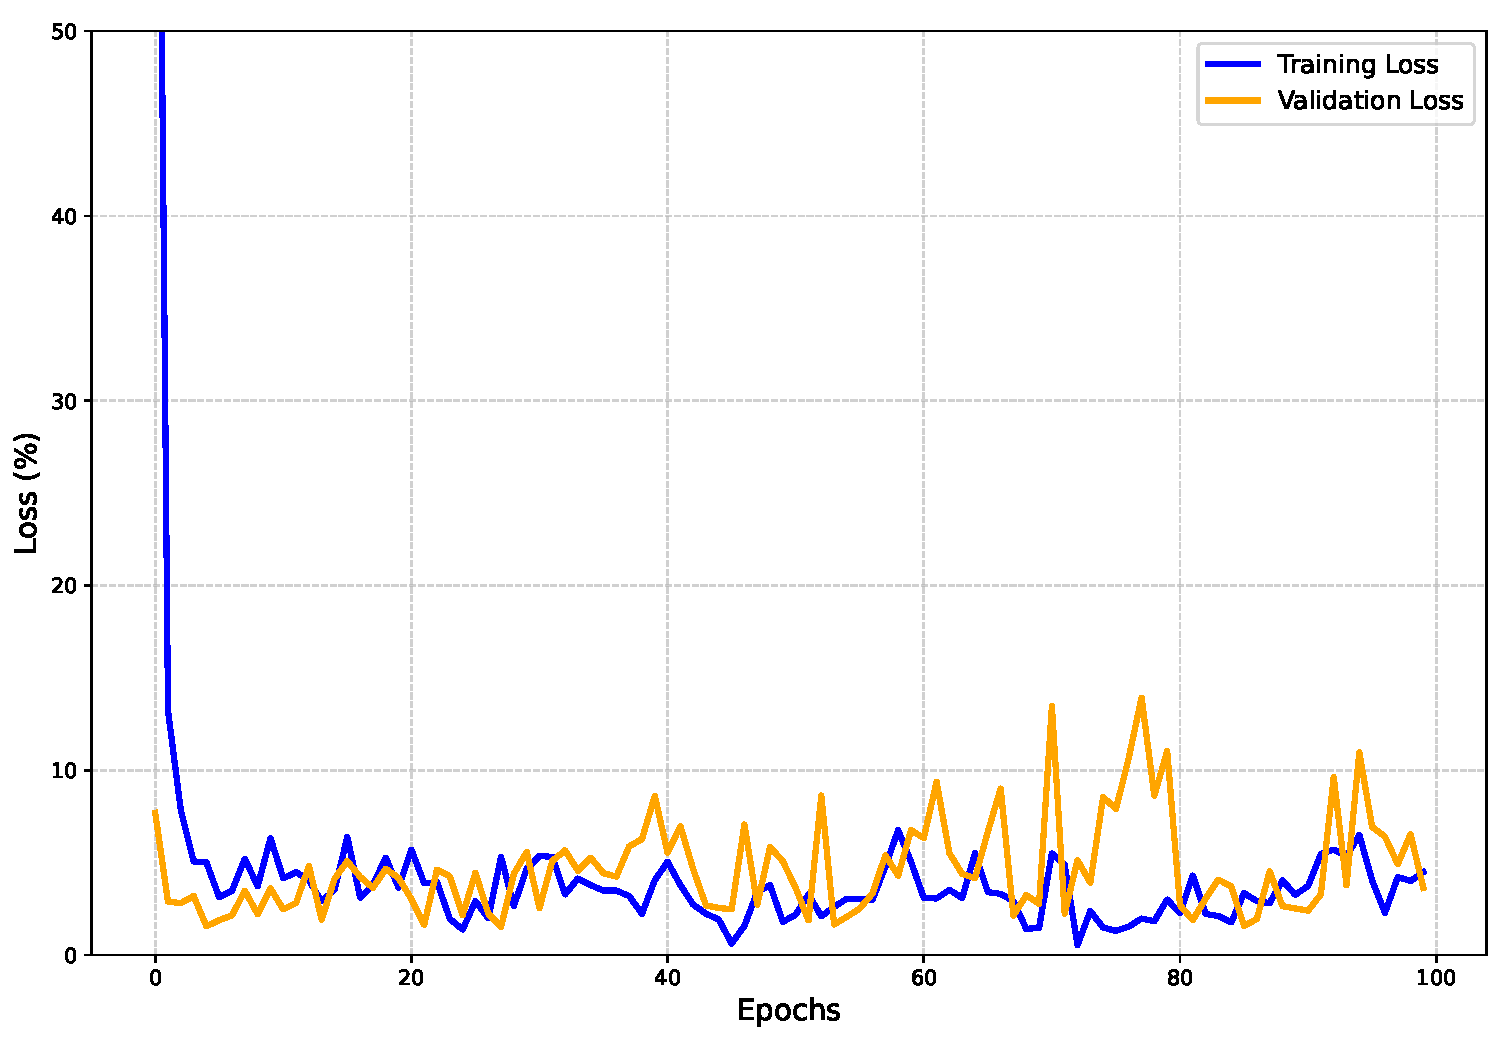
\includegraphics[height=8cm]{./fig/loss_curve.pdf} 
% \centering
% \caption{Loss Curve (ResNet-50 + Dense Layer)}
% \label{Loss_Curve}
% \end{figure}

Two distinct disease-gene networks (DGNs) were constructed using Cytoscape to visualize these relationships for matching up-regulated genes in Figure 4-1 and down-regulated genes in Figure 4-2, where disease nodes are source nodes and common gene nodes are target nodes \cite{b5}. In these networks, Orange-colored nodes are genes, pink-colored nodes are comorbidities and the center represents the main Beta-Thalassemia disease. Connections between diseases and genes are weighted using the Jaccard Coefficient. These DGNs illustrate the interconnections of beta-thalassemia with its comorbidities that showing how shared genes may drive common molecular mechanisms. The networks highlight that the strong genetic overlap is particularly with hypogonadism has 165 shared DEGs which suggesting a deep molecular relationship. Here arrhythmia (44 DEGs) also shows significant connectivity.\\

Some common genes that have connection with beta-thalassemia as well as multiple comorbidities. These genes are indicated as red color in the network of down regulated DGNs network that has significant molecular connection. These genes are listed below in Table 4-3 with their connected diseases. For example, gene 'DUSP4' and 'CD24' belongs to BT, ACM and as well as hypogonadism. That make our investigation more strong for the genetic connection between BT and its comorbidities.\\ 

\begin{table}[H]
    \centering
    \mycaption[Most significant gene that are common for multiple diseases for BT as well as it multiple comorbidities]{Most significant gene that are common for multiple diseases for BT as well as it multiple comorbidities}
    \begin{tabular}{|p{3cm}|p{8cm}|}
        \hline
        Gene Name & Connection with multiple diseases \\
        \hline
        DUSP4; CD24 & BT, ACM and hypogonadism \\
        \hline
        DTX4 & BT, hypothyroidism and hypogonadism \\
        \hline
        RRAGD & BT, ACM and diabetes \\
        \hline
        RAB20 & BT, hypothyroidism, hypogonadism and arrhythmia \\
        \hline
        ARID5B; RIN2; NFIL3; MAFB & BT, hypogonadism and diabetes \\
        \hline
        AKR1B1 & BT, arrhythmia and diabetes \\
        \hline
        CEBPD; CD14; MRC1 & BT, hypogonadism and diabetes \\
        \hline
        CXCR4; PHACTR1; LIN7A; PTGDS; FXYD6; SOCS1; SPON2; PTGER4; SLC1A3; CHI3L1 & BT, arrhythmia and hypogonadism \\
        \hline
        ZFYVE26; RRAD; SLCO5A1; MLPH & BT, PCOS and hypogonadism \\
        \hline
    \end{tabular}
    
    \label{tab:significant_genes}
\end{table}

\begin{figure}[H]
\centering
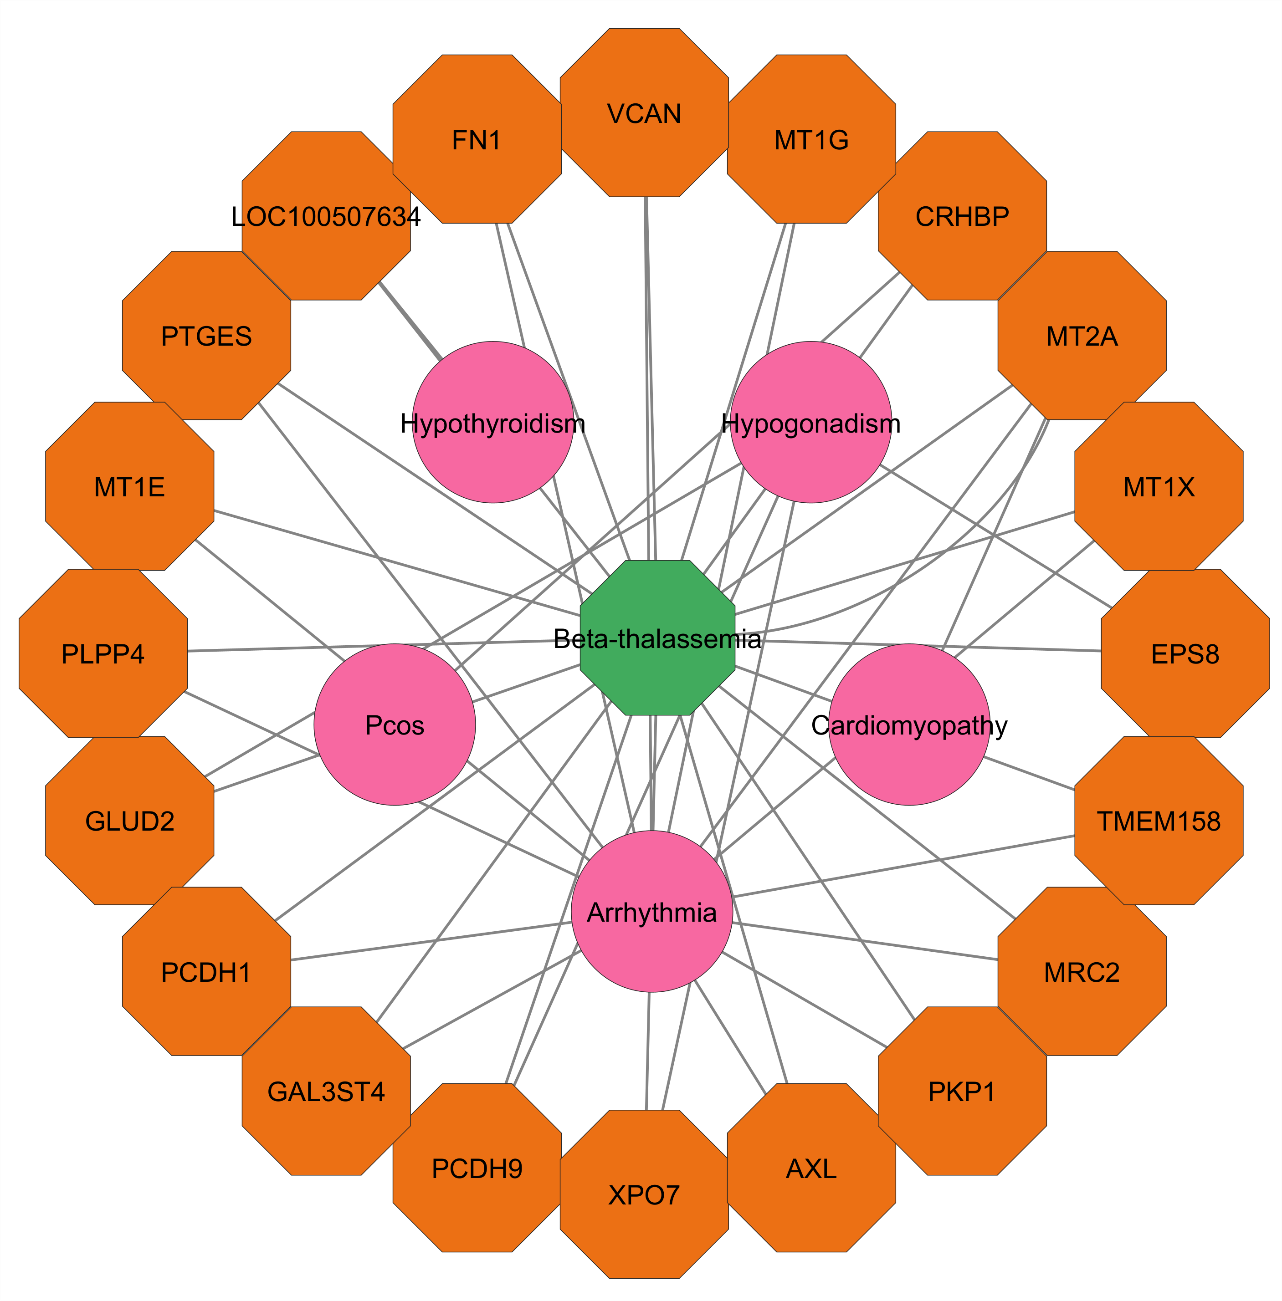
\includegraphics[height=14cm]{./fig/fig4_1.png} 
\centering
\caption{Loss Curve (DGNs network for up-regulation of common DEGs.  Orange-colored nodes are genes, pink-colored nodes are comorbidities and the center represents the beta-thalassemia.)}
\label{Loss_Curve}
\end{figure}

From Table 4-4, we can explore that genes those most significantly common for multiple diseases have must connection with 'hypogonadism'.  For ever genes in that table have a common connected disease that is'hypogonadism'. Thus this study can claim that hypogonadism has the evolutionary connection with beta-thalassemia that can affect beta-thalassemia patient.

\begin{figure}[H]
\centering
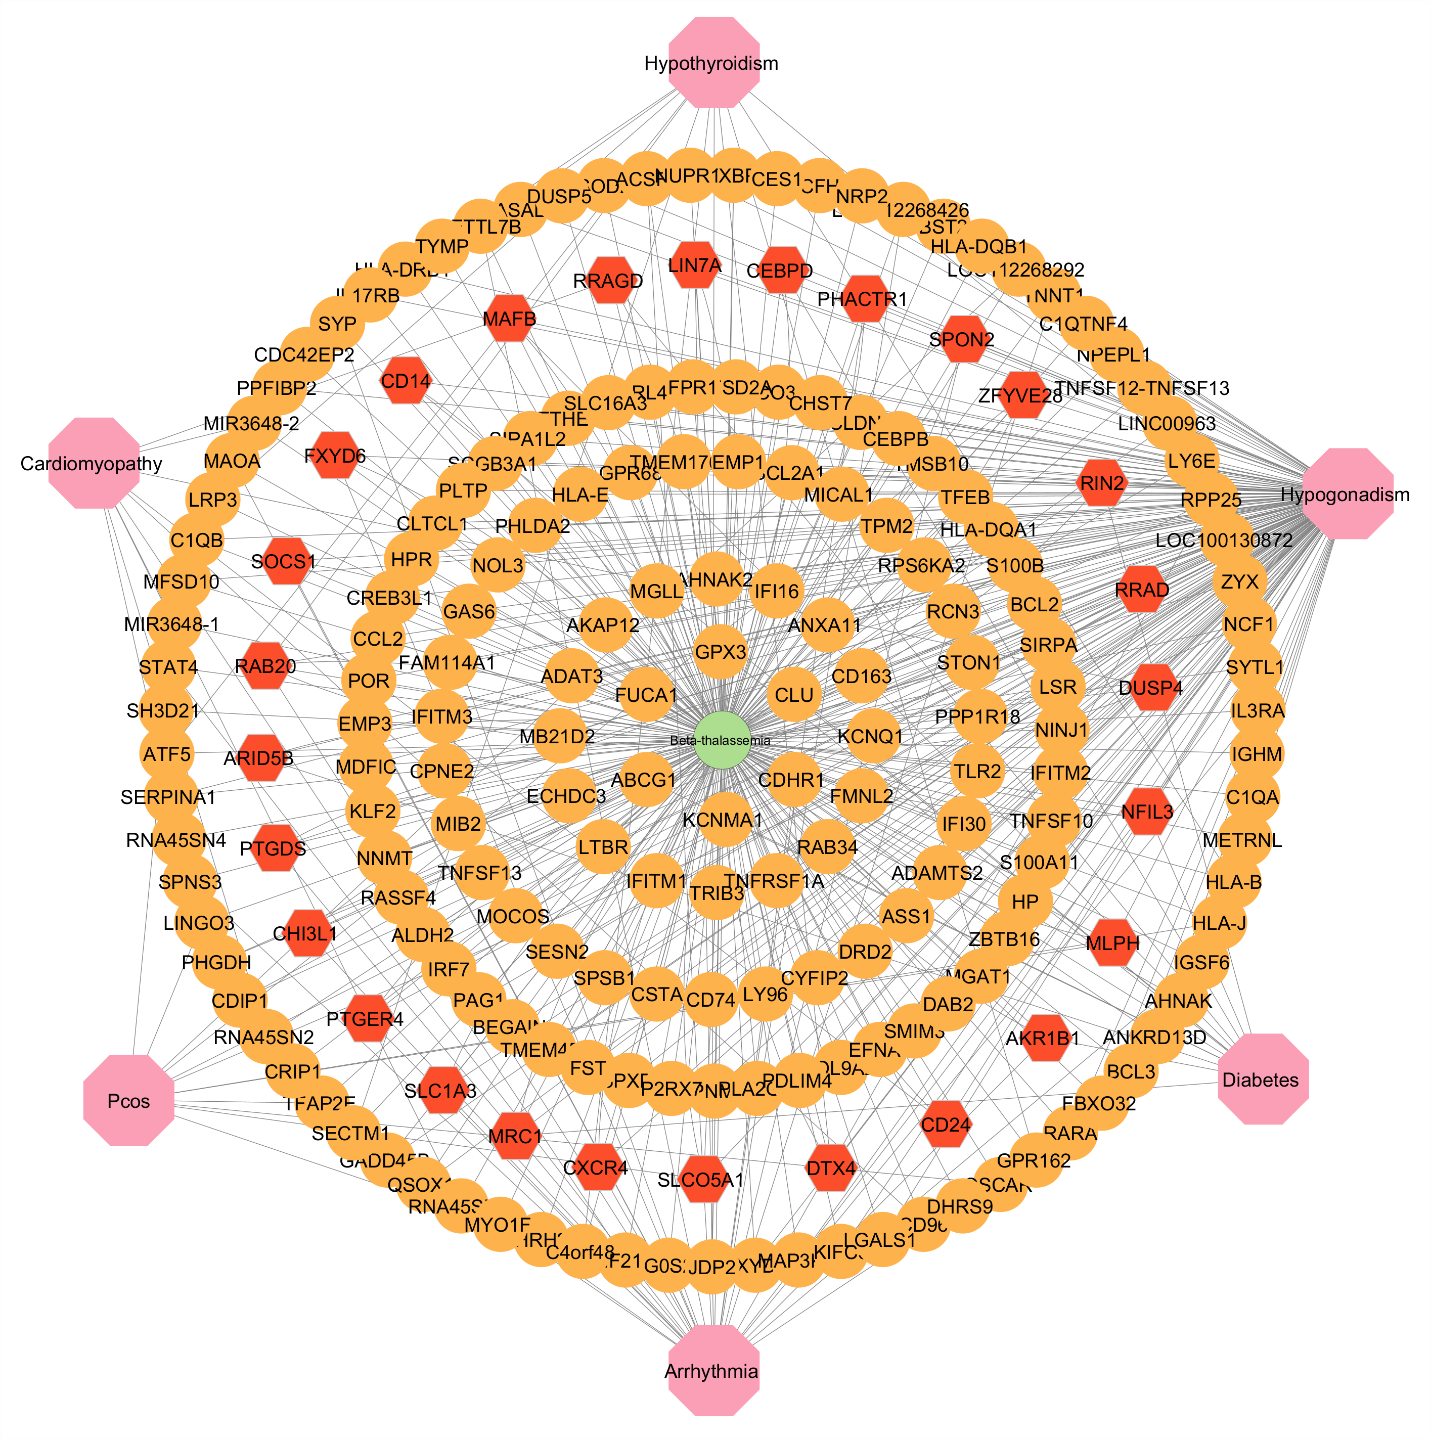
\includegraphics[height=14cm]{./fig/fig4_2.png} 
\centering
\caption{DGNs network for down-regulation of common DEGs.  Orange-colored nodes are genes, pink-colored nodes are comorbidities and the center represents the beta-thalassemia. Genes that are linked to several diseases are represented by the red color.}
\label{Loss_Curve}
\end{figure}

\section{Heatmap Visualization}
\label{sec:sec4_3}
This study visualizes a heat-map to represent the expression levels of differentially expressed genes among beta-thalassemia and its comorbidities. To visualize the expression level, we generate a heatmap using R's pheatmap package. Columns represent individual diseases like arrhythmia, PCOS, hypothyroidism, cardiomyopathy, hypogonadism, and T2D, and rows represent specific genes [6]. In this visualization, Red color visualizes down-regulated genes with lower expression, blue color visualizes up-regulated genes with higher expression, white or neutral colors represent no changes in expression.\\

\begin{figure}[H]
\centering
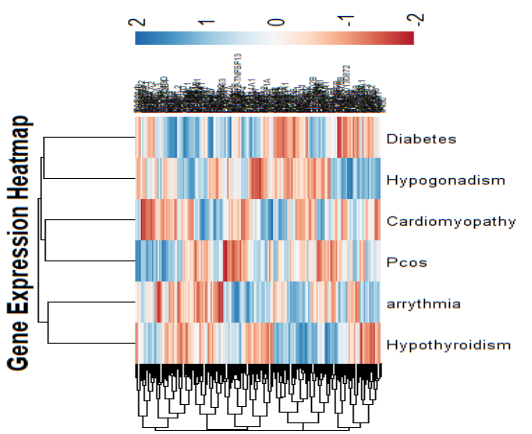
\includegraphics[height=12cm]{./fig/fig4_3.png} 
\centering
\caption{Heatmap visualization of gene expression.}
\label{Heatmap}
\end{figure}

The heatmap highlights clear differences in gene activity. For example, in hypogonadism, almost all genes are switched off (161 out of 165). And in arrhythmia, most are also turned down (30 out of 44). This pattern helps to underlying the causes of possibly related to iron overload or long-term anemia in beta-thalassemia. At the same time, 14 genes of arrhythmia are switched on, which could point to the activation of certain biological pathways. Overall, this visualization shows how gene expression varies across conditions and sets the stage for deeper pathway and interaction studies [6].


\section{Pathway and Functional Association Analysis}
\label{sec:sec4_3_3}

A Pathway is a sequence of molecular interactions that results in a specific change and product in a cell. It is a standard method for understanding the connection between complex diseases [6]. We investigated dysregulated gene pathways across four databases using Enrichr, such as Reactome, KEGG, WikiPathways and BioCarta. Significant pathways with adjusted p-value ≤ 0.05 were selected through statistical analysis.
From the analysis, we identified 11, 10, 13, 14, 13 and 13 significant pathways for hypothyroidism, hypogonadism, PCOS, T2D, ACM, and arrhythmia respectively. Significant pathways for each disease were identified and summarized in Table 4-5 to Table 4-10 and in Figure 4-4 to Figure 4-9 [7]:\\

\begin{table}[H]
    \centering
    \mycaption[Significant pathways of Hypothyroidism of shared DEGs]{Significant pathways of Hypothyroidism of shared DEGs}
    \begin{tabular}{|p{4cm}|p{3cm}|p{2cm}|p{4cm}|}
        \hline
        Significant Pathways & Gene Symbols & Adjusted P-Value & Most relevant disease for this pathway \\
        \hline
        Response of EIF2AK1 (HRI) to Heme Deficiency & ATF5 & 0.071135712 & Beta-thalassemia \\
        \hline
        Regulation of Innate Immune Responses to Cytosolic DNA & DTX4 & 0.071135712 & Particularly T2D, arrhythmia, ACM, and potentially thalassemia \\
        \hline
        Mitochondrial Unfolded Protein Response (UPRmt) & ATF5 & 0.071135712 & highly relevant to ACM, arrhythmia and diabetes \\
        \hline
        Nucleotide Salvage & TYMP & 0.074257875 & ACM and arrhythmia \\
        \hline
        Fluoropyrimidine Activity WP1601 & TYMP & 0.069079732 & T2D, ACM and arrhythmia \\
        \hline
        Type II Interferon Signaling WP619 & HLA-B & 0.069079732 & Most directly related to ACM and arrhythmia \\
        \hline
        Notch Signaling WP268 & DTX4 & 0.069079732 & ACM and arrhythmia \\
        \hline
        Proteasome Degradation WP183 & HLA-B & 0.069079732 & Particularly diabetes, cardiomyopathy, and arrhythmia \\
        \hline
        Allograft rejection & HLA-B & 0.110160639 & Cardiomyopathy \\
        \hline
        Graft-versus-host disease & HLA-B & 0.110160639 & diabetes \\
        \hline
        Autoimmune thyroid disease & HLA-B & 0.110160639 & Diabetes and hypothyroidism \\
        \hline
    \end{tabular}
    
    \label{tab:significant_pathways}
\end{table}

\begin{itemize}
    \item Reactome Database for Hypothyroidism
    \begin{itemize}
        \item The significant pathway ``Response of EIF2AK1 (HRI) to Heme Deficiency'' is specifically relevant to beta-thalassemia. It is a hallmark of BT, and the gene \textit{ATF5} is mainly responsible for thyroid problems.
        \item ``Regulation of Innate Immune Responses to Cytosolic DNA'' is particularly relevant to T2D, arrhythmia, ACM, and potentially to thalassemia. The gene \textit{DTX4} is responsible for beta-thalassemia.
        \item The significant pathway ``Mitochondrial Unfolded Protein Response (UPRmt)'' is highly relevant to ACM, arrhythmia, and diabetes, where the gene \textit{ATF5} may cause complications of BT.
        \item The ``Nucleotide Salvage'' pathway term significantly supports our findings with strong relevance to ACM and arrhythmia, where the responsible gene is \textit{TYMP}.
    \end{itemize}

    \item WikiPathways Database for Hypothyroidism
    \begin{itemize}
        \item For the pathway ``Type II Interferon Signaling WP619,'' the most directly related diseases are ACM and arrhythmia.
        \item For the pathway ``Proteasome Degradation WP183,'' the particularly relevant diseases are diabetes, cardiomyopathy, and arrhythmia. For both pathways, the gene \textit{HLA-B} is responsible.
    \end{itemize}

    \item KEGG Database for Hypothyroidism
    \begin{itemize}
        \item ``Allograft rejection,'' ``Graft-versus-host disease,'' and ``Autoimmune thyroid disease'' pathways involve the gene \textit{HLA-B}. These immune-related pathways are linked to cardiomyopathy, diabetes, and hypothyroidism.
    \end{itemize}
\end{itemize}

\begin{figure}[H]
\centering
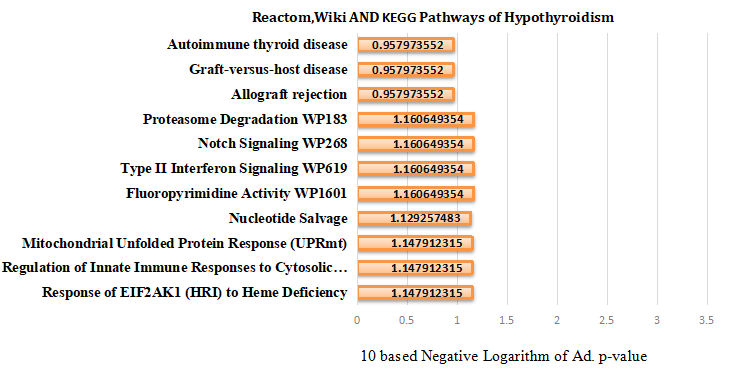
\includegraphics[height=7cm]{./fig/fig4_4.png} 
\centering
\caption{Graphical depiction of   pathways of Hypothyroidism}
\label{Significant_pathways_hypothyroidism}
\end{figure}

\newpage

\begin{longtable}{|p{2cm}|p{5cm}|p{2cm}|p{4cm}|}
    \caption[Significant pathways of Hypogonadism of shared DEGs]{Significant pathways of Hypogonadism of shared DEGs}\label{tab:significant_pathways_hypogonadism} \\
    \hline
    Significant Pathways & Gene Symbols & Adjusted P-Value & Most relevant disease for this pathway \\
    \hline
    Innate Immune System & CYFIP2; C1QB; C1QA;  SERPINA1;  CFH; HP; FPR1; LY96; DTX4;  SOCS1; IFI16; RPS6KA2; SIRPA;  QSOX1; CD14; S100A11;  DUSP4; S100B; HLA-E; BST2; P2RX7; BCL2; IRF7;  CHI3L1; TLR2 & 0.001030984 & Diabetes \\
    \hline
    Interferon Gamma Signaling & DSOCS1; IRF7; IFI30; HLA-DQA1; HLA-DRB1; HLA-E; HLA-DQB1 & 0.001785204 & Cardiomyopathy \\
    \hline
    Interferon Signaling & IFITM3; BST2; IFITM1; IFITM2;  SOCS1; IRF7; IFI30; HLA-DQA1; HLA-DRB1; HLA-E; HLA-DQB1 & 0.001798407 & Cardiomyopathy \\
    \hline
    Network Map Of SARS CoV 2 Signaling WP5115 & IFITM3; BST2; IFITM1;  CD163; CEBPB; CFH; HP;  TNFSF10;  CCL2;  CD14; HLA-DRB1 & 0.00125113 & T2D \\
    \hline
    Ebola Virus Infection In Host WP4217 & BST2; CLTCL1; IRF7; GAS6; HLA-DQA1; HLA-DRB1; HLA-E; HLA-DQB1 & 0.00125113 & Arrhythmia \\
    \hline
    Macrophage Markers WP4146 & CD74; CD163; CD14 & 0.002831209 & Cardiomyopathy \\
    \hline
    Tuberculosis & CD74; CEBPB; MRC1; BCL2;  CD14; HLA-DQA1; HLA-DRB1; TNFRSF1A; HLA-DQB1; TLR2 & 0.00027045 & T2D \\
    \hline
    Toxoplasmo-sis & SOCS1; BCL2; LY96; HLA-DQA1; HLA-DRB1; TNFRSF1A; HLA-DQB1; TLR2 & 0.000282742 & Diabetes and cardiomyopathy \\
    \hline
    Lipid and atherosclerosis & TNFSF10; BCL2; IRF7; MIB2;  LY96; CCL2; CD14; SOD2;  TNFRSF1A; TLR2 & 0.0005613633 & Arrhythmia \\
    \hline
    NF-kappa B signaling pathway & GADD45B; BCL2A1; BCL2;  LY96; CD14; LTBR; TNFRSF1A & 0.000845249 & Diabetes \\
    \hline
\end{longtable}

Total ten significant pathways with adjusted p-value $\leq$ 0.05 were identified due to their relevance to hypogonadism pathophysiology \cite{6}. "Innate Immune System", "Interferon Gamma Signaling" and "Interferon Signaling" most significant pathways were selected from Reactome databases. "Network Map of SARS CoV 2 Signaling WP5115", "Ebola Virus Infection In Host WP4217" and "Macrophage Markers WP4146" were selected from WikiPathways databases. And the other four in the table 4-6 were selected from KEEG pathways. These significant pathways shows e relevance with our comorbidities that make a strong evidence for our findings.\\

\begin{figure}[H]
\centering
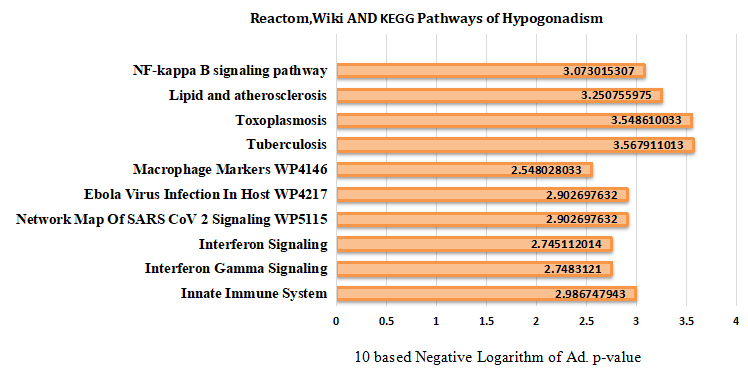
\includegraphics[height=7cm]{./fig/fig4_5.png} 
\centering
\caption{Graphical depiction of   pathways of Hypogonadism}
\label{Significant_pathways_hypogonadism}
\end{figure}

\newpage

\begin{longtable}{|p{4cm}|p{2.6cm}|p{2cm}|p{4cm}|}
    \caption[Significant pathways of PCOS of shared DEGs]{Significant pathways of PCOS of shared DEGs}\label{tab:significant_pathways_pcos} \\
    \hline
    Significant Pathways & Gene Symbols & Adjusted P-Value & Most relevant disease for this pathway \\
    \hline
    Cross-presentation of Particulate Exogenous Antigens (Phagosomes) & NCF1 & 0.119204664 & Diabetes \\
    \hline
    RHO GTPases Activate NADPH Oxidases & NCF1 & 0.12696123 & Diabetes \\
    \hline
    Detoxification of Reactive Oxygen Species & NCF1 & 0.12696123 & Diabetes \\
    \hline
    GPCR Ligand Binding & CRHBP;HRH2 & 0.14928425 & Hypogonadism, hypothyroidism, diabetes, cardiomyopathy, and arrhythmia \\
    \hline
    Signaling by Receptor Tyrosine Kinases & NCF1;RRAD & 0.151294003 & Arrhythmia \\
    \hline
    AGE RAGE Pathway WP2324 & NCF1 & 0.094169866 & T2D and cardiovascular \\
    \hline
    Urotensin II Mediated Signaling WP5158 & NCF1 & 0.094169866 & Diabetes and cardiomyopathy \\
    \hline
    Osteoclast differentiation & NCF1;OSCAR & 0.041730274 & Most relevant to diabetes and potentially related to thalassemia \\
    \hline
    Gastric acid secretion & HRH2 & 0.16687814 & Particularly Diabetes, Hypothyroidism, and potentially Thalassemia \\
    \hline
    Leishmaniasis & NCF1 & 0.16687814 & Arrhythmia and cardiomyopathy and potential indirect links to diabetes and thalassemia \\
    \hline
\end{longtable}

\begin{figure}[H]
\centering
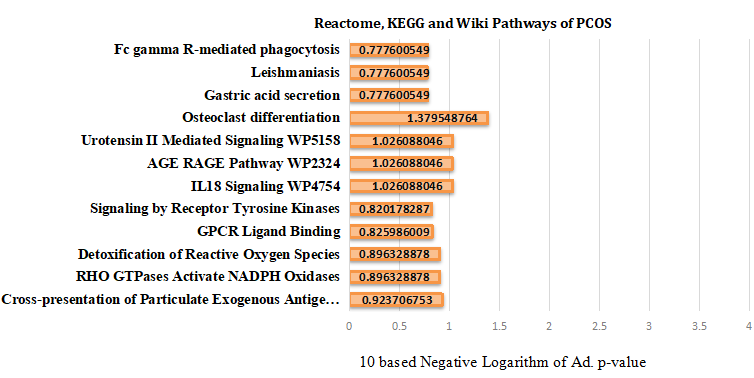
\includegraphics[height=7cm]{./fig/fig4_6.png} 
\centering
\caption{Graphical depiction of   pathways of PCOS.}
\label{Graphical depiction of   pathways of PCOS.}
\end{figure}


Pathway enrichment analysis for PCOS was performed by querying KEGG, Reactome, WikiPathways, and BioCarta databases. 
Below, we critically analyze these pathways to explain their biological significance and interconnections.

\begin{itemize}
    \item The GPCR ligand binding pathway, which includes \textit{CRHBP} (corticotropin-releasing hormone binding protein) and \textit{HRH2} (histamine receptor H2), plays an important role in several conditions such as hypogonadism, hypothyroidism, type~2 diabetes, cardiomyopathy, and arrhythmia. GPCR signaling helps control hormonal activity and inflammatory responses, which are directly tied to the hormonal disturbances seen in PCOS. In beta-thalassemia, iron overload interferes with GPCR-mediated hormonal pathways, which may intensify hormonal disturbances such as the rise in androgen levels often observed in PCOS.

    \item Osteoclast Differentiation involving \textit{NCF1} (neutrophil cytosolic factor 1) and \textit{OSCAR} (osteoclast-associated receptor) is most relevant to T2D and potentially beta-thalassemia. It governs bone remodeling, which is disrupted in metabolic and hematologic disorders. Iron overload in beta-thalassemia may impair bone metabolism through oxidative stress, linking to PCOS's metabolic complications.

    \item ``RHO GTPases Activate NADPH Oxidases,'' ``Detoxification of Reactive Oxygen Species,'' ``AGE-RAGE Pathway,'' ``IL18 Signaling,'' ``Urotensin II Mediated Signaling,'' and ``Leishmaniasis'' are significant pathways primarily driven by \textit{NCF1}. These are linked to T2D, cardiomyopathy, arrhythmia, and indirectly to beta-thalassemia. They involve oxidative stress (\textit{NCF1} activates NADPH oxidases), inflammation (IL18 signaling), and metabolic dysfunction (AGE-RAGE pathway). The role of \textit{NCF1} in oxidative stress pathways aligns with beta-thalassemia's iron-induced reactive oxygen species (ROS) production.
\end{itemize}

\begin{table}[H]
\centering
\caption{Significant pathways of T2D of shared DEGs}
\label{tab:T2D_pathways}
\renewcommand{\arraystretch}{1.2} % spacing between rows
\small
\begin{tabularx}{\textwidth}{|X|X|c|X|}
\hline
\textbf{Significant Pathways} & \textbf{Gene Symbols} & \textbf{Adjusted P-Value} & \textbf{Most Relevant Disease for this Pathway} \\
\hline
Fructose Metabolism & AKR1B1 & 0.086097405 & Diabetes \\
\hline
Terminal Pathway of Complement & CLU & 0.086097405 & Diabetes \\
\hline
Ca\textsuperscript{2+} Activated K\textsuperscript{+} Channels & KCNMA1 & 0.086097405 & Diabetes, arrhythmias and ACM \\
\hline
HDL Remodeling & ABCG1 & 0.086097405 & Cardiomyopathy \\
\hline
FTO Obesity Variant Mechanism WP3407 & ARID5B & 0.067455203 & Diabetes and PCOS \\
\hline
Macrophage Markers WP4146 & CD14 & 0.067455203 & Diabetes \\
\hline
Circadian Rhythm Genes WP3594 & NFIL3; KCNMA1 & 0.067455203 & Arrhythmia \\
\hline
Tuberculosis & MRC1; CD14 & 0.095231698 & Diabetes \\
\hline
Lipid and Atherosclerosis & CD14; ABCG1 & 0.095231698 & Diabetes and arrhythmias \\
\hline
Galactose Metabolism & AKR1B1 & 0.099417263 & Hypogonadism, diabetes and cardiomyopathy \\
\hline
Toll-Like Receptor Pathway (Homo sapiens, h\_tollPathway) & CD14 & 0.026965134 & Diabetes \\
\hline
Inactivation of Gsk3 by AKT causes accumulation of $\beta$-catenin in Alveolar Macrophages (Homo sapiens, h\_gsk3Pathway) & CD14 & 0.026965134 & Diabetes \\
\hline
\end{tabularx}
\end{table}

\begin{figure}[H]
\centering
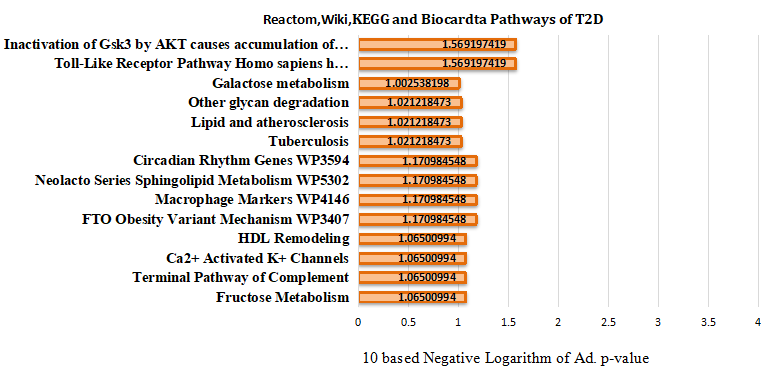
\includegraphics[height=7cm]{./fig/fig4_7.png} 
\centering
\caption{ Graphical depiction of   pathways of T2D.}
\label{ Graphical depiction of   pathways of T2D.}
\end{figure}

\begin{itemize}
    \item Fructose Metabolism and Galactose Metabolism pathways, both driven by \textit{AKR1B1} (aldo-keto reductase family 1 member B1), are highly relevant to T2D. In addition, Galactose Metabolism is also relevant to hypogonadism and cardiomyopathy. These pathways regulate sugar metabolism, which is critical in the insulin resistance profile of T2D. In beta-thalassemia, iron overload may exacerbate oxidative stress and upregulate \textit{AKR1B1} to handle sugar metabolites.

    \item Macrophage Markers and Toll-Like Receptor Pathway involve \textit{CD14}. Iron accumulation in beta-thalassemia likely triggers \textit{CD14}-mediated inflammation through TLR signaling.

    \item Tuberculosis and Lipid and Atherosclerosis pathways involve \textit{MRC1} (mannose receptor C-type 1), \textit{CD14}, and \textit{ABCG1} (ATP-binding cassette subfamily G member 1). These pathways govern immune responses and lipid metabolism. Iron overload in beta-thalassemia may disrupt lipid homeostasis (\textit{ABCG1}) and immune regulation (\textit{MRC1}, \textit{CD14}), thereby promoting atherosclerosis and inflammation in T2D.
\end{itemize}


\begin{table}[H]
\centering
\caption{Significant pathways of Arrhythmogenic Cardiomyopathy (ACM) of shared DEGs}
\label{tab:ACM_pathways}
\small\renewcommand{\arraystretch}{1.2} % increase row height 
for readability
\begin{tabularx}{\textwidth}{|X|X|c|X|}
\hline
\textbf{Significant Pathways} & \textbf{Gene Symbols} & \textbf{Adjusted P-Value} & \textbf{Most Relevant Disease for this Pathway} \\
\hline
Metallothioneins Bind Metals & \textit{MT2A} & 0.12931125 & Diabetes and cardiomyopathy \\
\hline
ERKs Are Inactivated & \textit{DUSP4} & 0.12931125 & Cardiomyopathy \\
\hline
Response to Metal Ions & \textit{MT2A} & 0.12931125 & Diabetes \\
\hline
ERK MAPK Targets & \textit{DUSP4} & 0.12931125 & Diabetes \\
\hline
mTORC1-mediated Signalling & \textit{RRAGD} & 0.12931125 & Diabetes \\
\hline
Zinc Homeostasis (WP3529) & \textit{MT2A} & 0.065424906 & Diabetes and hypogonadism \\
\hline
Target Of Rapamycin Signaling (WP1471) & \textit{RRAGD} & 0.065424906 & Diabetes and cardiomyopathy \\
\hline
Copper Homeostasis (WP3286) & \textit{MT2A} & 0.068235169 & Cardiomyopathy and arrhythmia \\
\hline
Endoderm Differentiation (WP2853) & \textit{DUSP4} & 0.082642753 & Diabetes \\
\hline
Mineral Absorption & \textit{MT2A} & 0.122298814 & T2D \\
\hline
Hematopoietic Cell Lineage & \textit{CD24} & 0.122298814 & Beta-thalassemia \\
\hline
Autophagy & \textit{RRAGD} & 0.122298814 & ACM \\
\hline
Regulation of MAP Kinase Pathways Through Dual Specificity Phosphatases (Homo sapiens, h\_dspPathway) & \textit{DUSP4} & 0.004940043 & Diabetes and cardiomyopathy \\
\hline
\end{tabularx}
\end{table}


\begin{itemize}
    \item \textbf{Metallothioneins Bind Metals}, \textbf{Response to Metal Ions}, \textbf{Copper Homeostasis}, and \textbf{Mineral Absorption} are driven by \textit{MT2A} (metallothionein 2A). \textit{MT2A} regulates metal ion homeostasis, particularly zinc and copper, thereby protecting against oxidative stress. Iron overload in beta-thalassemia likely induces oxidative stress, upregulating \textit{MT2A} to mitigate metal toxicity.

    \item \textbf{ERKs Are Inactivated}, \textbf{ERK MAPK Targets}, and \textbf{Regulation of MAP Kinase Pathways} involve \textit{DUSP4}, which regulates cell proliferation and stress responses. Iron-induced oxidative stress in beta-thalassemia may suppress \textit{DUSP4}, leading to dysregulated MAPK signaling.

    \item \textbf{Target of Rapamycin Signaling} and \textbf{Autophagy} are driven by \textit{RRAGD}. These pathways regulate mTORC1 signaling and autophagy, which are critical for cellular homeostasis and stress responses. In beta-thalassemia, iron overload may impair autophagy via \textit{RRAGD} dysregulation, leading to protein aggregation and cardiac damage in ACM.
\end{itemize}

\begin{figure}[H]
\centering
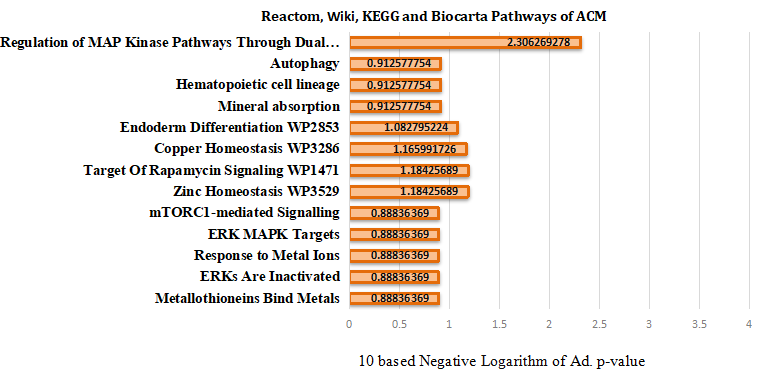
\includegraphics[height=7cm]{./fig/fig4_8.png} 
\centering
\caption{Graphical depiction of   pathways of ACM.}
\label{Graphical depiction of   pathways of ACM.}
\end{figure}

\begin{longtable}{|p{4cm}|p{5cm}|p{2cm}|p{4cm}|}
    \caption[Significant pathways of Arrhythmia of shared DEGs]{Significant pathways of Arrhythmia of shared DEGs}
    \label{tab:Arrhythmia_pathways} \\
    \hline
    \textbf{Significant Pathways} & \textbf{Gene Symbols} & \textbf{Adjusted P-Value} & \textbf{Most Relevant Disease for this Pathway} \\
    \hline
      \renewcommand{\arraystretch}{1.2} % spacing between rows
    \small
    Metallothioneins Bind Metals & \textit{MT2A; MT1G; MT1X; MT1E} & 1.362354723 & T2D and ACM \\
    \hline
    Response to Metal Ions & \textit{MT2A; MT1G; MT1X; MT1E} & 0.0000020563 & Diabetes \\
    \hline
    Neurotransmitter Release Cycle & \textit{MAOA; SLC1A3; LIN7A} & 0.013131521 & Diabetes \\
    \hline
    Synthesis of Prostaglandins (PG) and Thromboxanes (TX) & \textit{PTGDS; PTGES} & 0.02499481 & Arrhythmia \\
    \hline
    Zinc Homeostasis (WP3529) & \textit{MT2A; MT1G; MT1X; MT1E} & 0.0001265177 & Diabetes and hypogonadism \\
    \hline
    Prostaglandin Synthesis and Regulation (WP98) & \textit{PTGER4; AKR1B1; PTGDS; PTGES} & 0.0001577216 & Diabetes \\
    \hline
    Copper Homeostasis (WP3286) & \textit{MT2A; MT1G; MT1X; MT1E} & 0.000174674 & Arrhythmia and cardiomyopathy \\
    \hline
    Mineral Absorption & \textit{MT2A; MT1G; MT1X; MT1E} & 0.000644711 & Diabetes \\
    \hline
    JAK-STAT Signaling Pathway & \textit{SOCS1; IL3RA; STAT4} & 0.113203704 & ACM \\
    \hline
    Pathways in Cancer & \textit{PTGER4; IL3RA; STAT4; FN1; CXCR4} & 0.113203704 & Hypogonadism, diabetes, arrhythmia, cardiomyopathy \\
    \hline
    Eicosanoid Metabolism (Homo sapiens, h\_eicosanoidPathway) & \textit{PTGER4; PTGES} & 0.018593144 & Diabetes \\
    \hline
    Pertussis Toxin-Insensitive CCR5 Signaling in Macrophage (Homo sapiens, h\_Ccr5Pathway) & \textit{CXCR4} & 0.083487378 & Diabetes \\
    \hline
    CXCR4 Signaling Pathway (Homo sapiens, h\_cxcr4Pathway) & \textit{CXCR4} & 0.083487378 & Diabetes \\
    \hline
\end{longtable}

\begin{itemize}
    \item \textbf{Synthesis of Prostaglandins (PG) and Thromboxanes (TX)} and \textbf{Prostaglandin Synthesis and Regulation} involve \textit{PTGDS}, \textit{PTGES}, \textit{PTGER4}, and \textit{AKR1B1}, and are strongly linked to arrhythmia and diabetes. These pathways regulate prostaglandin synthesis, which influences inflammation and vascular function critical to cardiac rhythm. Iron overload in beta-thalassemia may enhance prostaglandin-mediated inflammation, contributing to the cardiac stress seen in arrhythmia.

    \item \textbf{Copper Homeostasis} is driven by metallothionein genes, including \textit{MT2A}, \textit{MT1G}, \textit{MT1X}, and \textit{MT1E}. This pathway regulates copper ion balance and protects against oxidative stress. Iron accumulation in beta-thalassemia likely induces oxidative stress, upregulating metallothioneins to mitigate metal toxicity, which is critical for protecting cardiac tissue in arrhythmia.

    \item \textbf{Pathways in Cancer} involve \textit{PTGER4}, \textit{IL3RA}, \textit{STAT4}, \textit{FN1}, and \textit{CXCR4}. These govern cell proliferation and signaling pathways often dysregulated in chronic diseases. In beta-thalassemia, iron-induced oxidative stress may dysregulate \textit{FN1} and \textit{CXCR4}, contributing to cardiac remodeling in arrhythmia and overlapping with metabolic (diabetes) and endocrine (hypogonadism) dysfunction.

    \item \textbf{JAK-STAT Signaling Pathway} is linked to arrhythmia and ACM. This pathway involves \textit{SOCS1}, \textit{IL3RA}, and \textit{STAT4}, which regulate cytokine signaling and immune responses. Chronic inflammation from beta-thalassemia's iron overload may activate JAK-STAT signaling, contributing to cardiac inflammation in arrhythmia.
\end{itemize}

\begin{figure}[H]
\centering
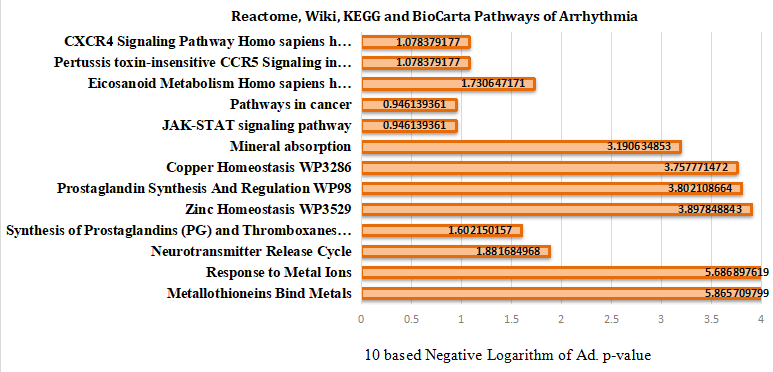
\includegraphics[height=7cm]{./fig/fig4_9.png} 
\centering
\caption{ Graphical depiction of   pathways of Arrhythmia.}
\label{ Graphical depiction of   pathways of Arrhythmia.}
\end{figure}

\section{Gene Ontology (GO) Analysis}
\label{sec:sec4_5}
Gene Ontology (GO) analysis provides a structured framework to characterize the molecular functions, biological processes, and cellular components of genes which offering insights into their roles in disease mechanisms \cite{b5}. We performed GO analysis with Enrichr by querying the GO Biological Process and Human Phenotype Ontology (HPO) databases \cite{b6}. This analysis describes detailed in Table 4-11 to Table 4-16 to explain the molecular and phenotypic connections linking these diseases.

\begin{table}[H]
\centering
\caption{Gene Ontological significant pathways of Hypothyroidism of shared DEGs}
\label{tab:Hypothyroidism_GO}
\renewcommand{\arraystretch}{1.2} % spacing between rows
\small
\begin{tabularx}{\textwidth}{|c|X|c|X|X|}
\hline
\textbf{Term} & \textbf{Name} & \textbf{Adjusted P-Value} & \textbf{Genes} & \textbf{Most Relevant Disease for this Pathway} \\
\hline
GO:0002664 & Regulation of T Cell Tolerance Induction & 0.060741016 & \textit{HLA-B} & Diabetes \\
\hline
GO:0007219 & Notch Signaling Pathway & 0.085112911 & \textit{DTX4} & Cardiomyopathy \\
\hline
HP:0001824 & Weight loss & 0.044703647 & \textit{HLA-B; TYMP} & T2D \\
\hline
HP:0002027 & Abdominal pain & 0.044703647 & \textit{HLA-B; TYMP} & T2D and cardiomyopathy \\
\hline
HP:0004395 & Malnutrition & 0.044703647 & \textit{TYMP} & Diabetes and hypothyroidism \\
\hline
HP:0100653 & Optic neuritis & 0.044703647 & \textit{HLA-B} & Diabetes and arrhythmias \\
\hline
\end{tabularx}
\end{table}

\subsection*{1. GO Terms: }
\begin{enumerate}
    \item The term \textbf{GO:0002664} is driven by \textit{HLA-B}, which regulates immune tolerance and is particularly relevant to diabetes. In beta-thalassemia (BT), iron overload may disrupt \textit{HLA-B}-mediated immune regulation, contributing to autoimmune thyroid dysfunction, a hallmark of hypothyroidism.
    
    \item The Notch Signaling Pathway (\textbf{GO:0007219}) involves \textit{DTX4}. This pathway governs cell differentiation and is linked to cardiomyopathy. Its relevance to hypothyroidism suggests that iron-induced stress in BT may affect thyroid cell differentiation, potentially exacerbating hormonal imbalances.
\end{enumerate}

\subsection*{2. HPO Terms: }
\begin{enumerate}
    \item The phenotype \textbf{Weight Loss} (\textbf{HP:0001824}) is associated with T2D. This reflects metabolic dysregulation, which may also occur in hypothyroidism due to thyroid hormone imbalances. Iron overload in BT could exacerbate metabolic stress, contributing to weight loss.
    \item \textbf{Abdominal Pain} (\textbf{HP:0002027}) is linked to T2D and cardiomyopathy. This phenotype may indicate systemic inflammation or gastrointestinal complications in hypothyroidism, potentially driven by BT's iron toxicity.
    \item \textbf{Malnutrition} (\textbf{HP:0004395}) is relevant to diabetes and hypothyroidism. This term suggests nutrient absorption issues and may be linked to systemic effects of iron overload on metabolism in BT patients.
    \item \textbf{Optic Neuritis} (\textbf{HP:0100653}), involving the gene \textit{HLA-B} (adjusted $p$-value = 0.045), is associated with diabetes and arrhythmia. This inflammatory phenotype may reflect immune dysregulation in hypothyroidism, possibly amplified by chronic inflammation in BT.
\end{enumerate}


\begin{table}[H]
\centering
\caption{Gene Ontological significant pathways of Hypogonadism of shared DEGs.}
\renewcommand{\arraystretch}{1.0} % for row spacing
\small
\begin{tabularx}{\textwidth}{|l|X|c|X|X|}
\hline
\textbf{Term} & \textbf{Name} & \textbf{Adjusted p-value} & \textbf{Genes} & \textbf{Most relevant disease for this pathway} \\
\hline
GO:0050727 & Regulation of Inflammatory Response & 0.004340401 & \textit{PTGER4; LGALS1; IFI16; NINJ1; SIRPA; METRNL; PLA2G7; MGLL; TNFRSF1A; TLR2} & Diabetes \\
\hline
GO:0032753 & Positive Regulation of Interleukin-4 Production & 0.013597802 & \textit{CEBPB; RARA; HLA-E} & Diabetes \\
\hline
GO:0032675 & Regulation of Interleukin-6 Production & 0.013795602 & \textit{C1QTNF4; CD74; GPNMB; SIRPA; GAS6; TLR2} & Diabetes \\
\hline
GO:0097193 & Intrinsic Apoptotic Signaling Pathway & 0.014095553 & \textit{CEBPB; BCL2A1; IFI16; BCL2; TRIB3; CD24} & Diabetes \\
\hline
HP:0000099 & Glomerulonephritis & 0.042357015 & \textit{C1QB; C1QA; CFH} & Diabetes \\
\hline
HP:0100539 & Periorbital edema & 0.099130412 & \textit{ADAMTS2; RIN2; TNFRSF1A} & Hypothyroidism \\
\hline
HP:0002725 & Systemic lupus erythematosus & 0.099691906 & \textit{C1QB; C1QA} & T2D \\
\hline
HP:0001287 & Meningitis & 0.156489906 & \textit{IGHM; BCL2; HLA-DRB1} & T2D \\
\hline
\end{tabularx}
\end{table}


Using Enrichr, we queried the GO and HPO databases to identify four significant GO terms and four HPO terms \cite{6}.

\subsection*{1. GO Terms:}
\begin{enumerate}
    \item \textbf{Regulation of Inflammatory Response}: Involving genes such as \textit{PTGER4}, \textit{LGALS1}, \textit{SIRPA}, and \textit{TLR2}. This pathway underscores inflammation modulation in hypogonadism. Iron overload in beta-thalassemia (BT) likely triggers \textit{TLR2}-mediated inflammatory responses, contributing to gonadal dysfunction through chronic inflammation.
    
    \item \textbf{Positive Regulation of Interleukin-4 Production}: Driven by \textit{CEBPB}, \textit{RARA}, and \textit{HLA-E}. This pathway regulates IL-4, an anti-inflammatory cytokine. Dysregulation suggests an altered immune balance in hypogonadism, potentially exacerbated by BT's oxidative stress affecting hormonal regulation.
    
    \item \textbf{Regulation of Interleukin-6 Production}: Involving \textit{CD74}, \textit{GPNMB}, and \textit{TLR2}. This pathway indicates IL-6-driven inflammation. Iron-induced oxidative stress in BT may amplify IL-6, disrupting gonadal function in hypogonadism.
\end{enumerate}

\subsection*{2. HPO Terms:}
\begin{enumerate}
    \item \textbf{Glomerulonephritis}: Linked to diabetes but relevant to hypogonadism, involving \textit{C1QB}, \textit{C1QA}, and \textit{CFH}. This phenotype suggests inflammatory damage, potentially driven by BT's systemic inflammation affecting gonadal tissues.
    
    \item \textbf{Systemic Lupus Erythematosus}: Involving \textit{C1QB} and \textit{C1QA}, this term indicates autoimmune-like mechanisms that may contribute to hypogonadism's immune dysregulation in the context of BT.
    
    \item \textbf{Meningitis}: Linked to \textit{IGHM}, \textit{BCL2}, and \textit{HLA-DRB1}. This phenotype suggests broader inflammatory effects.
\end{enumerate}

\begin{table}[H]
\centering
\caption{Gene Ontological significant pathways of PCOS of shared DEGs.}
\renewcommand{\arraystretch}{1.0} % for row spacing
\small
\begin{tabularx}{\textwidth}{|l|X|c|X|X|}
\hline
\textbf{Term} & \textbf{Name} & \textbf{Adjusted p-value} & \textbf{Genes} & \textbf{Most relevant disease for this pathway} \\
\hline
GO:0030316 & Osteoclast Differentiation & 0.046477967 & \textit{OSCAR} & Diabetes \\
\hline
HP:0005406 & Recurrent bacterial skin infections & 0.04671673 & \textit{NCF1} & Diabetes \\
\hline
HP:0100721 & Mediastinal lymphadenopathy & 0.04671673 & \textit{NCF1} & Diabetes and ACM \\
\hline
HP:0006510 & Chronic obstructive pulmonary disease & 0.04671673 & \textit{NCF1} & Diabetes \\
\hline
HP:0000230 & Gingivitis & 0.04671673 & \textit{NCF1} & Diabetes \\
\hline
\end{tabularx}
\end{table}

In GO pathway analysis of PCOS, it involves 1 GO terms and 4 HP terms. We can determined from table 4-13 that all HP term is involving the NCF1 gene. The GO term Osteoclast Differentiation highlights bone metabolism dysregulation that linking PCOS to BT's iron overload through OSCAR-mediated oxidative stress with overlaps in diabetes's metabolic profile. All HPO terms is driven by NCF1 that emphasize inflammatory and immune dysregulation which suggesting that iron-induced oxidative stress in BT amplifies NCF1-mediated inflammation and contributing to PCOS's clinical phenotypes like infections and systemic inflammation.

\begin{table}[H]
\centering
\caption{Gene Ontological significant pathways of T2D of shared DEGs.}
\renewcommand{\arraystretch}{1.0} % for row spacing
\small
\begin{tabularx}{\textwidth}{|l|X|c|X|X|}
\hline
\textbf{Term} & \textbf{Name} & \textbf{Adjusted p-value} & \textbf{Genes} & \textbf{Most relevant disease for this pathway} \\
\hline
GO:0043691 & Reverse Cholesterol Transport & 0.00445197 & \textit{CLU; ABCG1} & Diabetes \\
\hline
GO:1902003 & Regulation of Amyloid-Beta Formation & 0.007020347 & \textit{CLU; ABCG1} & T2D \\
\hline
GO:0140467 & Integrated Stress Response Signaling & 0.007020347 & \textit{MAFB; CEBPD} & T2D \\
\hline
GO:0030301 & Cholesterol Transport & 0.0144153 & \textit{CLU; ABCG1} & Diabetes \\
\hline
HP:0009120 & Aplasia/Hypoplasia involving the sinuses & 0.0455770 & \textit{FUCA1} & Diabetes \\
\hline
HP:0000970 & Anhidrosis & 0.045577 & \textit{FUCA1} & Diabetes \\
\hline
HP:0003541 & Urinary glycosaminoglycan excretion & 0.04557702 & \textit{FUCA1} & Diabetes \\
\hline
HP:0000815 & Hypergonadotropic hypogonadism & 0.0532044 & \textit{RIN2} & Hypogonadism and PCOS \\
\hline
\end{tabularx}
\end{table}

Four significant GO terms and four HPO terms with adjusted p-value $\leq 0.05$ were identified for T2D. The GO terms, including ``Reverse Cholesterol Transport'' and ``Regulation of Amyloid-Beta Formation,'' are driven by \textit{CLU} and \textit{ABCG1} genes, highlighting lipid metabolism and stress response. These terms link T2D to beta-thalassemia's (BT) iron-induced metabolic dysregulation, and ``Integrated Stress Response Signaling'' driven by \textit{MAFB} and \textit{CEBPD} genes suggests cellular stress.  

HPO terms like ``Aplasia/Hypoplasia Involving the Sinuses,'' ``Anhidrosis,'' and ``Urinary Glycosaminoglycan Excretion'' involving \textit{FUCA1} indicate metabolic and inflammatory phenotypes. ``Hypergonadotropic Hypogonadism'' connects to hypogonadism and PCOS, reflecting shared endocrine disruptions. These findings underscore iron overload's role in T2D's metabolic and inflammatory pathology, suggesting potential therapeutic targets such as lipid-modulating agents.

\begin{table}[H]
\centering
\caption{Gene Ontological significant pathways of ACM of shared DEGs.}
\small
\renewcommand{\arraystretch}{1.1}
\begin{tabularx}{\textwidth}{|l|X|c|X|X|}
\hline
\textbf{Term} & \textbf{Name} & \textbf{Adjusted p-value} & \textbf{Genes} & \textbf{Most relevant disease for this pathway} \\
\hline
GO:0072311 & Glomerular Epithelial Cell Differentiation & 0.037250334 & \textit{CD24} & Diabetes \\
\hline
GO:0072112 & Podocyte Differentiation & 0.037250334 & \textit{CD24} & T2D \\
\hline
GO:0030856 & Regulation of Epithelial Cell Differentiation & 0.039402171 & \textit{CD24} & Cardiomyopathy and arrhythmia \\
\hline
GO:0043627 & Response to Estrogen & 0.048014194 & \textit{CD24} & Diabetes \\
\hline
HP:0000243 & Trigonocephaly & 0.064644186 & \textit{CD96} & Hypothyroidism \\
\hline
HP:0000057 & Clitoromegaly & 0.064644186 & \textit{CD96} & PCOS \\
\hline
HP:0010318 & Aplasia/Hypoplasia of the abdominal wall musculature & 0.074611621 & \textit{CD96} & Diabetes \\
\hline
\end{tabularx}
\end{table}

Four significant GO terms and three HPO terms were identified for ACM. The GO terms, including ``Glomerular Epithelial Cell Differentiation,'' ``Podocyte Differentiation,'' and ``Regulation of Epithelial Cell Differentiation,'' are driven by \textit{CD24}, highlighting epithelial cell regulation relevant to cardiomyopathy and arrhythmia. These terms suggest iron overload in beta-thalassemia (BT) disrupts \textit{CD24}-mediated cellular differentiation, contributing to cardiac tissue remodeling. HPO terms like ``Trigonocephaly,'' ``Clitoromegaly,'' and ``Aplasia/Hypoplasia of the abdominal wall musculature'' are driven by \textit{CD96}, reflecting developmental and endocrine phenotypes connecting to hypothyroidism, PCOS, and diabetes, and may indicate systemic effects of iron toxicity. These findings suggest therapeutic targets such as anti-inflammatory or hormonal modulators. \\


\begin{table}[H]
\centering
\caption{Gene Ontological significant pathways of Arrhythmia of shared DEGs.}

\renewcommand{\arraystretch}{1.0}
\small
\begin{tabularx}{\textwidth}{|l|X|c|X|X|}
\hline
\textbf{Term} & \textbf{Name} & \textbf{Adjusted p-value} & \textbf{Genes} & \textbf{Most relevant disease for this pathway} \\
\hline
GO:0042093 & T-helper Cell Differentiation & 0.024608573 & \textit{PTGER4; STAT4} & Diabetes \\
\hline
GO:0006692 & Prostanoid Metabolic Process & 0.024608573 & \textit{PTGDS; PTGES} & T2D \\
\hline
GO:0007399 & Nervous System Development & 0.067160207 & \textit{VCAN; AXL; FN1; CXCR4; PCDH1} & PCOS \\
\hline
HP:0100820 & Glomerulopathy & 0.137761059 & \textit{STAT4; FN1} & Diabetes \\
\hline
HP:0003323 & Progressive muscle weakness & 0.137761059 & \textit{TNNT1} & Hypothyroidism \\
\hline
HP:0100614 & Myositis & 0.137761059 & \textit{STAT4} & Arrhythmia \\
\hline
\end{tabularx}
\end{table}

Three significant GO terms and three HPO terms were identified for arrhythmia. The GO terms, including ``T-helper Cell Differentiation'' and ``Prostanoid Metabolic Process,'' are driven by \textit{PTGER4}, \textit{STAT4}, \textit{PTGDS}, and \textit{PTGES}, highlighting immune and inflammatory processes. Iron overload in BT drives \textit{STAT4}-mediated immune dysregulation and \textit{PTGDS}/\textit{PTGES}-related prostaglandin synthesis. ``Nervous System Development,'' involving \textit{VCAN}, \textit{AXL}, \textit{FN1}, \textit{CXCR4}, and \textit{PCDH1}, indicates neural influences relevant to PCOS and potentially links to autonomic nervous system effects on cardiac rhythm. HPO terms like ``Glomerulopathy'' and ``Myositis'' reflect inflammatory phenotypes directly relevant to arrhythmia, while ``Progressive Muscle Weakness'' connects to hypothyroidism, suggesting muscle-related cardiac impacts.\\

The GO and HPO analyses, conducted using Enrichr between BT and its comorbidities, reveal shared molecular and phenotypic mechanisms driven by iron overload. GO terms underscore immune and metabolic pathways, while HPO terms reflect clinical phenotypes linked to endocrine, inflammatory, and cardiac complications. These findings indicate that iron-induced oxidative stress and inflammation are central to comorbidity development in beta-thalassemia. The overlap across diseases suggests shared therapeutic targets, such as anti-inflammatory or iron-chelating agents, to mitigate these conditions. This integrative analysis provides a molecular framework for understanding beta-thalassemia's systemic impact, guiding future research and clinical strategies.


\section{Protein-Protein Interactions Analysis}
\label{sec:sec4_6}
Protein-Protein Interaction (PPI) analysis is a cornerstone of systems biology, enabling the prediction of protein functions and potential drug targets through molecular interactions \cite{b7}. Using the STRING database with a high confidence score (900), we analyzed PPIs of the shared differentially expressed genes (DEGs) between BT and its comorbidities. We constructed PPI networks using the Network Analyst platform as visualized in Figure 4-10. The identified hub proteins play critical roles in immune regulation, inflammation, and cellular stress that linking BT iron overload to endocrine and cardiac comorbidities. The high connectivity of CD74 and BCL2 suggests their central role in inflammatory and apoptotic pathways. These findings highlight potential therapeutic targets, such as anti-inflammatory or immune-modulating agents, for managing comorbidities in beta-thalassemia. Network Stats of our findings in Table 4-17. We identified mainly 86 seeds from where top 15 hub proteins are given in Table 4-18. \\

\begin{table}[H]
    \centering
    \mycaption[Network Stats information of PPI analysis]{Network Stats information of PPI analysis}
    \begin{tabular}{|p{4cm}|p{3cm}|}
        \hline
        \textbf{Description} & \textbf{Value} \\
        \hline
        Number of nodes: & 219 \\
        \hline
        Number of edges: & 462 \\
        \hline
        Average node degree: & 4.22 \\
        \hline
        Avg. local clustering coefficient: & 0.344 \\
        \hline
    \end{tabular}
    \label{tab:network_stats_ppi}
\end{table}

\textbf{Degree}: The degree of a gene or node in a PPI network is the number of direct interactions through edges with other genes/proteins. It measures how connected a gene is within the network. A high degree indicates that a gene is a hub that interacting with many other proteins and suggesting it plays a central role in biological processes.\\

\textbf{Betweenness}: It centrality measures how often a gene or node lies on the shortest paths between other pairs of nodes in the network. It quantifies a gene's role as a "bridge" or mediator in facilitating interactions between other proteins. A high betweenness centrality indicates that a gene is crucial for connecting different parts of the network, controlling the flow of information or signals, and is often pivotal in coordinating biological functions.\\

\begin{table}[H]
    \centering
    \small
    \mycaption[Identify Hub protein information from PPIs analysis]{Identify Hub protein information from PPIs analysis}
    \renewcommand{\arraystretch}{1.2} % spacing between rows
    \begin{tabular}{|c|p{2.5cm}|c|c|}
        \hline
        Serial No. & Hub Protein & Degree & Betweeness \\
        \hline
        1 & CD74 & 132 & 139810.9 \\
        \hline
        2 & BCL2 & 61 & 122437.4 \\
        \hline
        3 & FN1 & 56 & 126043.7 \\
        \hline
        4 & TNFRSF1A & 41 & 41685.53 \\
        \hline
        5 & CXCR4 & 41 & 76314.66 \\
        \hline
        6 & TLR2 & 34 & 46163.96 \\
        \hline
        7 & CEBPB & 29 & 53645.13 \\
        \hline
        8 & HLA-DRB1 & 25 & 21809.87 \\
        \hline
        9 & IRF7 & 25 & 20416.19 \\
        \hline
        10 & SOCS1 & 24 & 27432.88 \\
        \hline
        11 & HLA-B & 23 & 13507.96 \\
        \hline
        12 & RARA & 22 & 21166.3 \\
        \hline
        13 & CLTCL1 & 22 & 18312 \\
        \hline
        14 & HLA-E & 20 & 20407.77 \\
        \hline
        15 & CYFIP2 & 20 & 15689.23 \\
        \hline
    \end{tabular}
    
    \label{tab:hub_protein_ppi}
\end{table}

\begin{figure}[H]
    \centering
    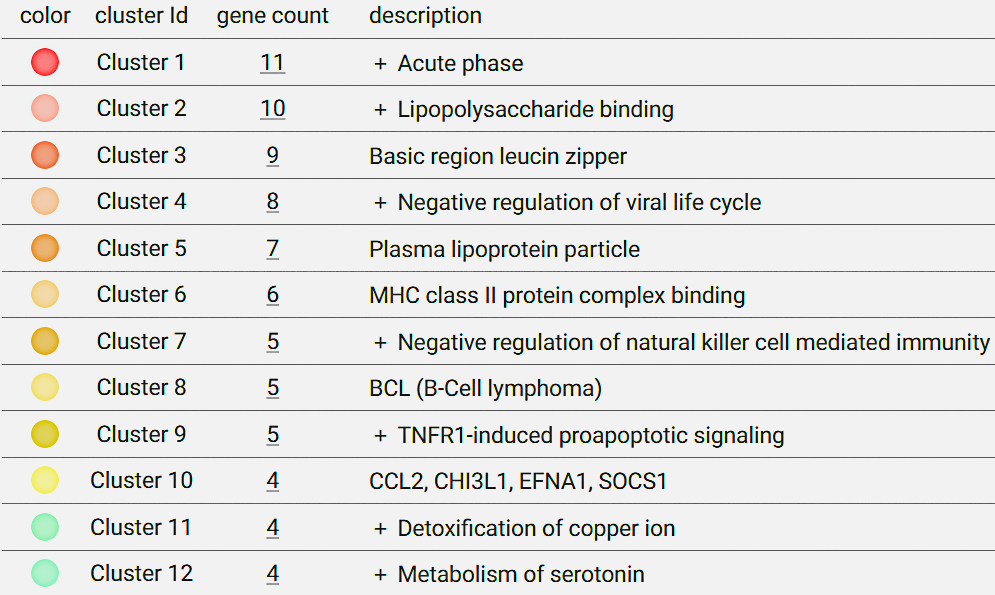
\includegraphics[height=7cm]{./fig/fig4_10.png}
    \centering
    \caption{Clusters information's of PPI networks of hub proteins of beta-thalassemia and comorbidities.}
    \label{PPI networks of hub proteins}
\end{figure}


The PPI network is shown below in Figure 4.11:

\begin{figure}[H]
    \centering
    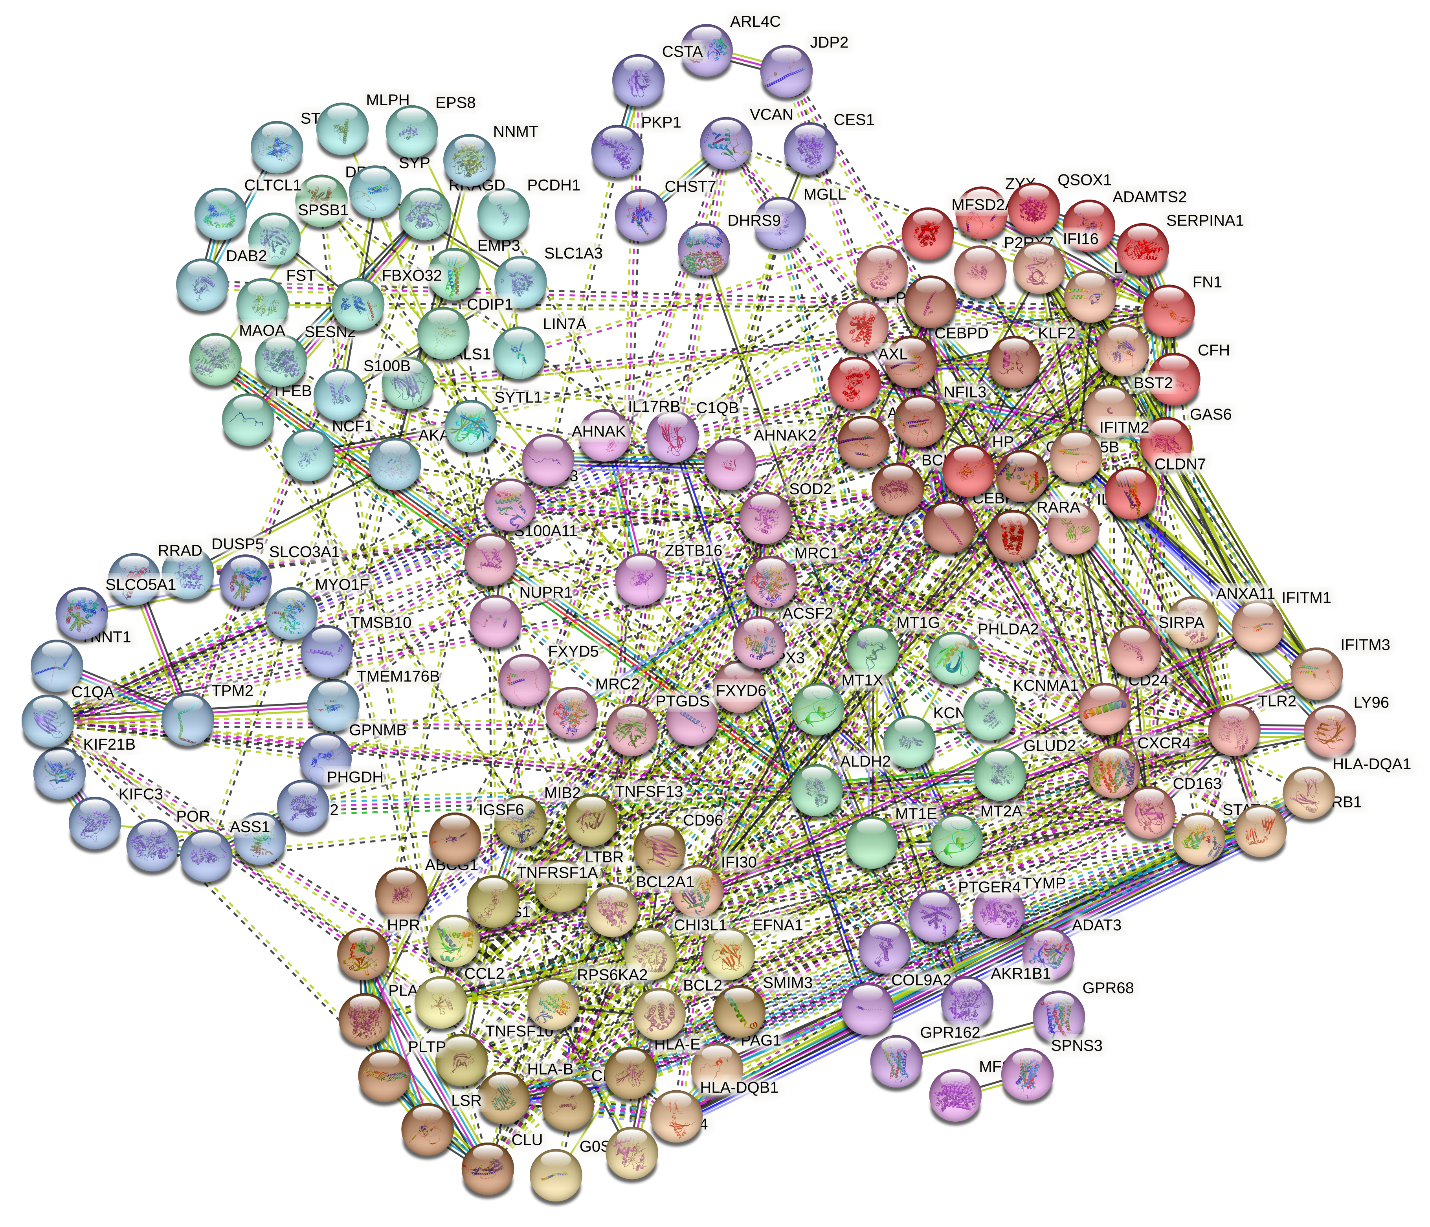
\includegraphics[height=10cm]{./fig/fig4_11.png}
    \centering
    \caption{PPI networks of hub proteins of beta-thalassemia and comorbidities.}
    \label{PPI networks of hub proteins of beta-thalassemia and comorbidities.}
\end{figure}

\begin{itemize}
    \item \textbf{CD74} is a central hub in the PPI network. \textit{CD74} manages MHC class II antigen processing, guiding peptide-free complexes to endosomal/lysosomal systems. In beta-thalassemia, it drives immune dysregulation worsened by iron overload, fueling inflammation in hypogonadism, T2D, and arrhythmia. Its link to MIF amplifies systemic inflammation across these comorbidities.
    
    \item \textbf{BCL2} is a key hub in the PPI network that blocks apoptosis by regulating mitochondrial permeability and caspase activity. In beta-thalassemia, it counters iron-driven cell death in cardiac and endocrine (hypogonadism) tissues.
    
    \item \textbf{FN1} is involved in cell adhesion, motility, and extracellular matrix (ECM) remodeling. In BT, iron overload disrupts ECM integrity, impacting cardiac and endocrine tissues. \textit{FN1}'s role in osteoblast compaction and collagen deposition connects to bone metabolism issues observed in PCOS. 
    
    \item \textbf{CXCR4} is a hub protein that mediates cell migration and inflammation via CXCL12/SDF-1 signaling. Its role in nervous system development (Table 4-16) and inflammation links to arrhythmia and PCOS, where iron-induced oxidative stress amplifies inflammatory responses. 
    
    \item \textbf{TLR2} (Toll-like receptor 2) mediates innate immune responses to bacterial lipoproteins, driving NF-kappa-B activation and inflammation. In BT, \textit{TLR2} contributes to chronic inflammation, exacerbating comorbidities like hypogonadism, T2D, and arrhythmia. 
    
    \item \textbf{SOCS1} is a hub protein that regulates cytokine signaling via JAK/STAT pathways, inhibiting IL-6 and interferon-gamma signaling. Its role in immune modulation is critical for BT's inflammatory environment, impacting T2D and ACM. 
    
    \item \textbf{HLA-B} (HLA class I histocompatibility antigen) regulates immune tolerance. Its high connectivity in the PPI network suggests it contributes to autoimmune aspects of hypothyroidism and T2D in BT. 
    
    \item \textbf{NCF1} drives oxidative stress via NADPH oxidase, exacerbating inflammation in beta-thalassemia and contributing to PCOS's inflammatory phenotypes.
\end{itemize}


\section{Protein-Drug Interactions Analysis}
\label{sec:sec4_7}

Protein-Drug Interaction (PDI) analysis was conducted to identify potential therapeutic drug targets for beta-thalassemia and its comorbidities by leveraging the Network Analyst platform and the DrugBank database \cite{8}. Two PDI networks were constructed based on shared differentially expressed genes (DEGs) identified by uploading 231 genes in Network Analyst. \\

The first PDI network comprises 20 hub genes, represented as circles, including \textit{C1QA} and \textit{C1QB}, with squares indicating their interacting drug molecules. These hubs, part of the complement system, suggest potential anti-inflammatory drug targets to mitigate iron-induced immune dysregulation in comorbidities like T2D and arrhythmia. \\

The second PDI network includes 15 hub genes, highlighting \textit{PLA2G7} and \textit{CES1}, alongside their interacting drug molecules. \textit{PLA2G7} (platelet-activating factor acetylhydrolase) and \textit{CES1} (liver carboxylesterase 1) are linked to lipid metabolism and xenobiotic detoxification, respectively, pointing to therapeutic strategies for endocrine and cardiac complications. \\

These PDI networks are visualized in Figure 4-12 to reveal key molecular targets for drug development, emphasizing anti-inflammatory and metabolic modulators to address iron overload's systemic effects in beta-thalassemia comorbidities \cite{8}. \\

\begin{table}[H]
    \centering
    \mycaption[Information of drug interactions of PDI Subnetwork1]{Information of drug interactions of PDI Subnetwork1}
    \small
    \renewcommand{\arraystretch}{1.2} % spacing between rows
    \begin{tabular}{|c|p{3cm}|c|c|}
        \hline
        Serial No. & Drug Name & Degree & Betweeness \\
        \hline
        1 & C1QB & 18 & 76.5 \\
        \hline
        2 & C1QA & 18 & 76.5 \\
        \hline
        3 & Cetuximab & 2 & 0.05555556 \\
        \hline
        4 & Etanercept & 2 & 0.05555556 \\
        \hline
        5 & Adalimumab & 2 & 0.05555556 \\
        \hline
        6 & Abciximab & 2 & 0.05555556 \\
        \hline
        7 & Gemtuzumab ozogamicin & 2 & 0.05555556 \\
        \hline
        8 & Trastuzumab & 2 & 0.05555556 \\
        \hline
        9 & Rituximab & 2 & 0.05555556 \\
        \hline
        10 & Basiliximab & 2 & 0.05555556 \\
        \hline
    \end{tabular}
    
    \label{tab:drug_interactions_pdi}
\end{table}

\begin{figure}[H]
    \centering
    \begin{subfigure}[t]{0.48\textwidth}
        \centering
        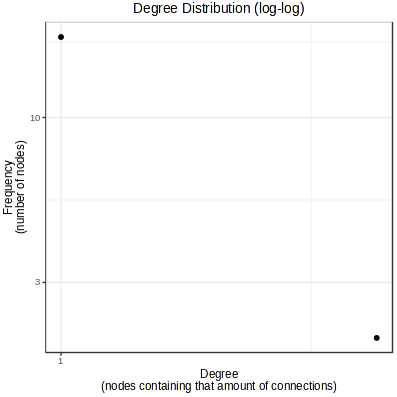
\includegraphics[width=\textwidth]{./fig/fig4_12_1.png}
        \label{fig:subnetwork1}
    \end{subfigure}
    \hfill
    \begin{subfigure}[t]{0.48\textwidth}
        \centering
        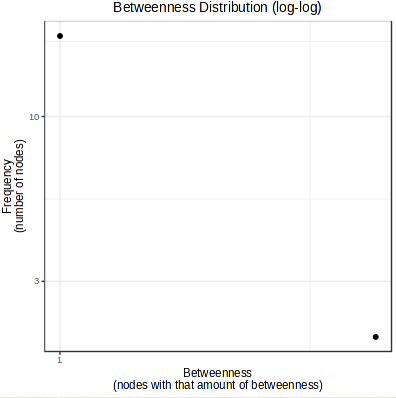
\includegraphics[width=\textwidth]{./fig/fig4_12_2.png}
        \label{fig:subnetwork2}
    \end{subfigure}
    \caption{Network Topology of Subnetwork1. }
    \label{fig:figure4-12}
\end{figure}

\begin{table}[H]
\centering
\caption{Information of drug interactions of PDI Subnetwork2.}
\label{tab:drug_interactions_subnet2}
\renewcommand{\arraystretch}{1.2} % spacing between rows
\small
\begin{tabularx}{\textwidth}{|c|X|c|c|}
\hline
\textbf{Serial No.} & \textbf{Drug Name} & \textbf{Degree} & \textbf{Betweenness} \\
\hline
1 & CES1 & 12 & 88 \\
\hline
2 & PLA2G7 & 2 & 13 \\
\hline
3 & (1R)-1,2,2-TRIMETHYLPROPYL (R)-METHYLPHOSPHINATE & 2 & 24 \\
\hline
4 & Oseltamivir & 1 & 0 \\
\hline
5 & L-Carnitine & 1 & 0 \\
\hline
6 & Probucol & 1 & 0 \\
\hline
7 & Hydroxy-Phenyl-Acetic Acid 8-Methyl-8-Aza-Bicyclo[3.2.1]Oct-3-Yl Ester & 1 & 0 \\
\hline
8 & Cholic Acid & 1 & 0 \\
\hline
9 & 4-Piperidino-Piperidine & 1 & 0 \\
\hline
10 & N-acetyl-alpha-neuraminic acid & 1 & 0 \\
\hline
\end{tabularx}
\end{table}


\begin{figure}[H]
    \centering
    \begin{subfigure}[t]{0.48\textwidth}
        \centering
        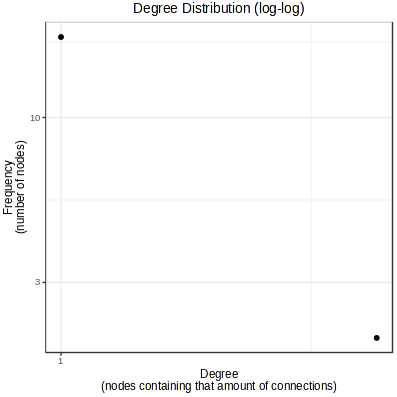
\includegraphics[width=\textwidth]{./fig/fig4_13_1.png}
        \label{fig:subnetwork1}
    \end{subfigure}
    \hfill
    \begin{subfigure}[t]{0.48\textwidth}
        \centering
        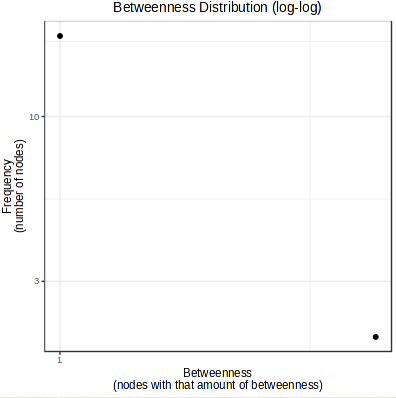
\includegraphics[width=\textwidth]{./fig/fig4_13_2.png}
        \label{fig:subnetwork2}
    \end{subfigure}
    \caption{Network Topology of Subnetwork2. }
    \label{fig:figure4-13}
\end{figure}

\begin{figure}[H]
    \centering
    \begin{subfigure}[t]{0.48\textwidth}
        \centering
        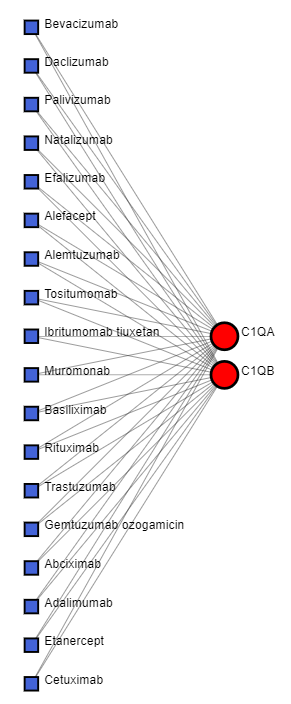
\includegraphics[height=20cm, keepaspectratio]{./fig/fig4_14_1.png}
        \label{fig:subnetwork1}
    \end{subfigure}
    \hfill
    \begin{subfigure}[t]{0.48\textwidth}
        \centering
        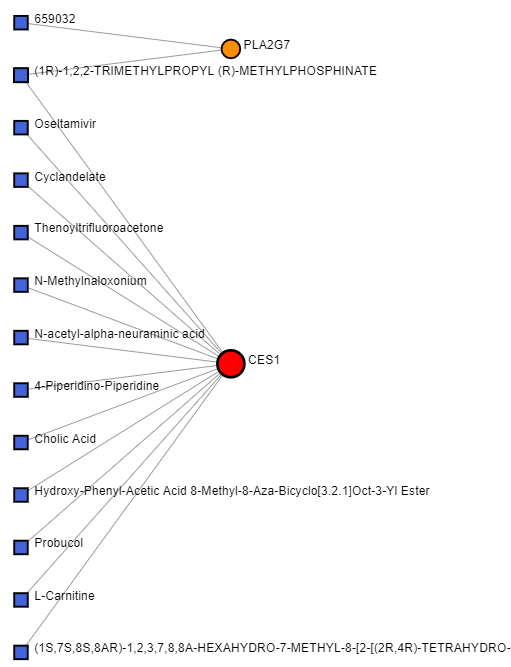
\includegraphics[height=20cm, width=8cm]{./fig/fig4_14_2.png}
        \label{fig:subnetwork2}
    \end{subfigure}
    \caption{PDI networks of drug proteins of beta-thalassemia and comorbidities.}
    \label{fig:figure4-14}
\end{figure}


\section{Results of Phylogenetic Analysis}
\label{sec:sec4_8}
Phylogenetic analysis enhances the understanding of the evolutionary relationships among genes, proteins and diseases \cite{8}. We constructed a phylogenetic tree for beta-thalassemia and its comorbidities to illustrate the associative relationships among them by using Molecular Evolutionary Genetics Analysis (MEGA) tools and FASTA sequences of nucleotide datasets from NCBI \cite{8}. The phylogenetic tree shows the relationship between beta-thalassemia and the comorbidities including PCOS, T2D, hypogonadism, hypothyroidism, ACM and arrhythmia in Figure~\ref{fig:phylogenetic_tree}. The tree shows a strong evolutionary relationship between beta-thalassemia and hypogonadism as they belong to a common species.\\

\begin{figure}[H]
    \centering
    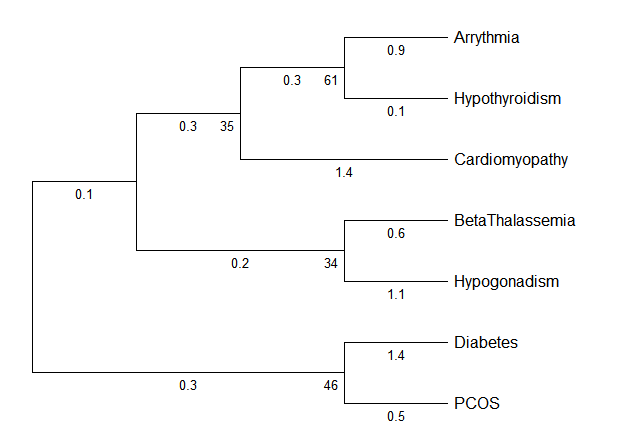
\includegraphics[height=10cm]{./fig/fig4_15.png}
    \centering
    \caption{Phylogenetic tree to illustrate associative evolutionary relationship between beta-thalassemia and its comorbidities.}
    \label{Phylogenetic tree to illustrate associative evolutionary relationship between beta-thalassemia and its comorbidities.}
\end{figure}

To validate our findings, we used two benchmark databases including dbGap and OMIM from Enrichr tools on the up-regulated and down-regulated genes of beta-thalassemia \cite{b9}. The analysis identified several drugs and diseases from which we identified twelve diseases whose genes are similar to the genes of beta-thalassemia. Among those identified diseases, our six selected comorbidities were present that support the validity of our study. The other six diseases may be the potential comorbidities of beta-thalassemia, T2D, hypothyroidism, hypogonadism, PCOS, arrhythmogenic cardiomyopathy and arrhythmia. To illustrate these associations, we constructed a drug-disease validation network using Cytoscape, as shown in Figure~\ref{fig:drug_disease_network} \cite{b10}.

\begin{figure}[H]
    \centering
    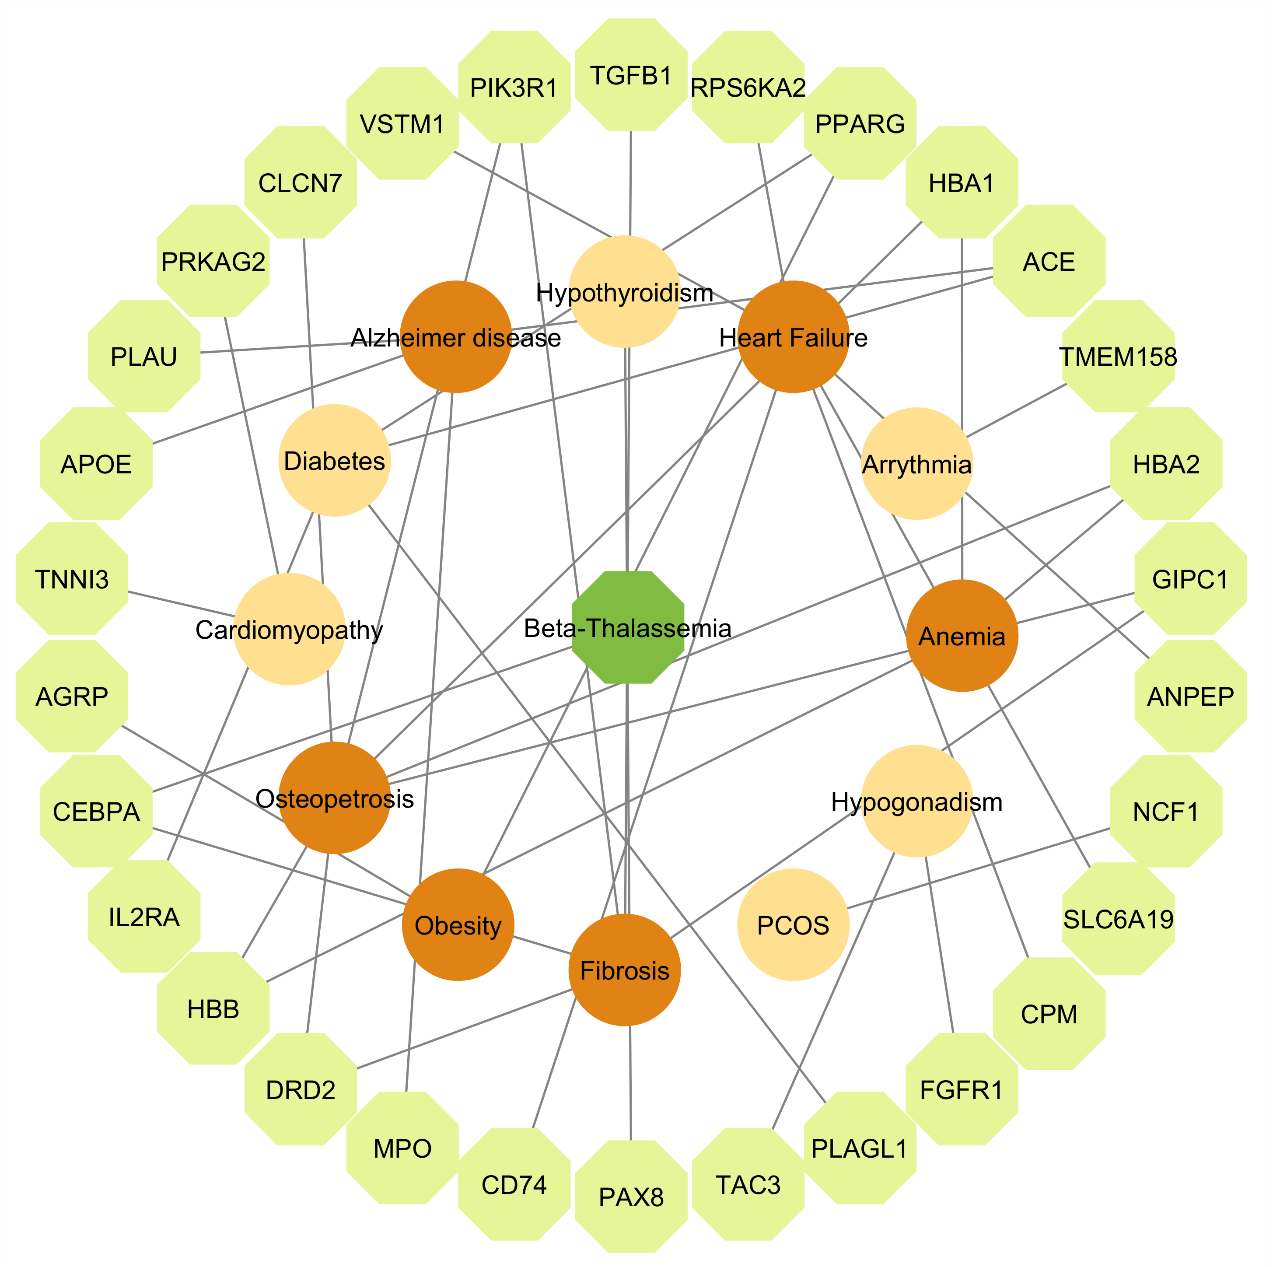
\includegraphics[height=10cm]{./fig/fig4_16.png}
    \centering
    \caption{Graphical representation of validation network of beta-thalassemia. Octagon shapes indicate the shared genes, circle shapes with brown color indicate our selected diseases and circle shapes with yellow-orange color represent our selected comorbidities.}
    \label{fig:drug_disease_network}
\end{figure}

\section{Discussion}
This chapter presents the comprehensive outcomes of the proposed investigation into beta-thalassemia and its comorbidities. We explored dysregulated genes, disease gene networks, signaling pathways, Gene Ontology (GO) and Human Phenotype Ontology (HPO) terms, Protein-Protein Interaction (PPI) networks, and Protein-Drug Interaction (PDI) networks in detail. Key findings reveal that iron overload drives inflammation, apoptosis, and metabolic dysregulation, linking beta-thalassemia to its comorbidities through hub genes and therapeutic targets such as in the PDI analysis.\\


The simulation environment effectively mapped the regulatory networks, identifying critical pathways which underpin the pathophysiological overlap across comorbidities. The phylogenetic tree illustrates associative patterns, suggesting stronger molecular ties between BT and hypogonadism. These results provide a solid foundation for future therapeutic strategies targeting iron overload and its systemic effects in beta-thalassemia.

